%%%%%%%%%%%%%%%%%%%%%%%%%%%%%%%%%%%%%%%%%%%%%%%%%%%%%%%%%%%%%%%%%
\chapter{EXPERIMENTAL SETUP AND METHODOLOGY}\label{ch:Ch3}
%%%%%%%%%%%%%%%%%%%%%%%%%%%%%%%%%%%%%%%%%%%%%%%%%%%%%%%%%%%%%%%%%
\vspace*{-12pt} % If no text above section, use this vspacing to lift the whole part to the proper starting point - SBÖ
%\section{Body Texts}
This chapter is devoted to explaining the experimental setup and the data obtained for the condition monitoring and diagnostics of the induction motor. Experiments were carried out in the General Purpose Industrial Motor Laboratory at WAT Motor Company facilities. During the studies, the faults related to the bearing, stator and rotor of the squirrel-cage induction motor were artificially created and their data were collected. The test system used in the study is shown in Figure \ref{experiment}.

\begin{figure}[h]
	\centering
	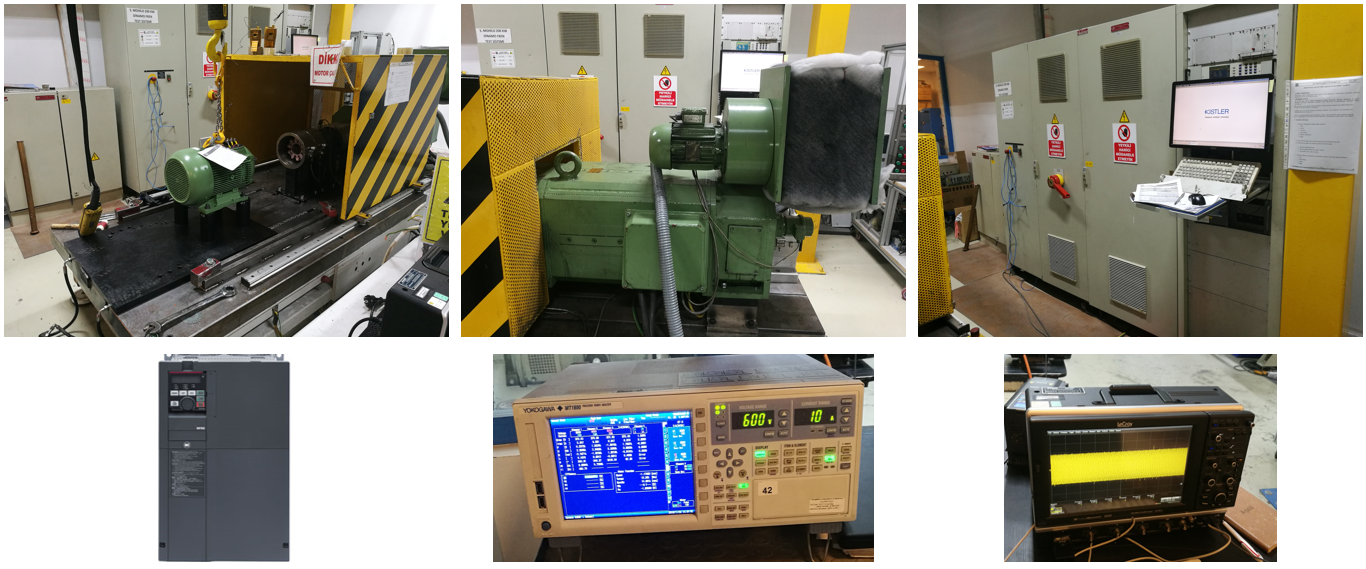
\includegraphics[width=400pt,keepaspectratio=true]{./fig/expsystem.PNG}
	% sekil3.eps: 0x0 pixel, 300dpi, 0.00x0.00 cm, bb=14 14 1155 740
	\caption{Experiment setup, courtesy of WAT Motor Co.}	
	\label{experiment}
\end{figure}

\begin{table*}[h]
	{\setlength{\tabcolsep}{12pt}
		\caption{Equipments used in experimental-setup.}
		\begin{center}
			\vspace{-6mm}
			\begin{tabular}{c}
				\hline \\[-2.45ex] \hline \\[-2.1ex]
				Equipment\\
				\hline \\[-1.8ex]
				Kistler 200 kW Dynamometer  \\
				Yokogawa Power Analyzer  \\
				Teledyne LeCroy Oscilloscope  \\
				WAT-11 kW Induction Motors   \\
				WAT-WF-80 General Purpose Variable Frequency Driver   \\
				\hline
			\end{tabular}
			\vspace{-6mm}
		\end{center}
		\label{Table3.1}}
\end{table*}

In the experimental studies, the stability of the system was tracked by monitoring the three-phase current and voltage signals on the power analyzer. One phase of the stator supply current of the motor was recorded with a current probe at a sampling frequency of 5 kHz for 10 seconds. In addition, the load torque acting on the motor and the rotor rotation speed of the motor were measured via the dynamometer system.

\begin{figure}[h]
	\centering
	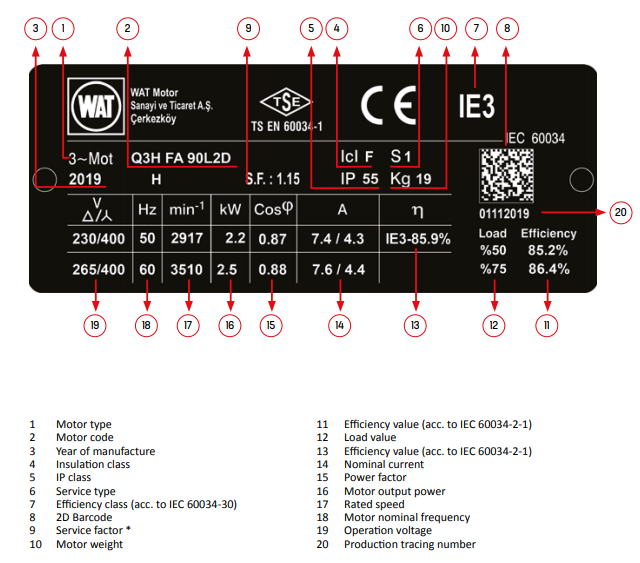
\includegraphics[width=250pt,keepaspectratio=true]{./fig/plate.PNG}
	% sekil3.eps: 0x0 pixel, 300dpi, 0.00x0.00 cm, bb=14 14 1155 740
	\caption{Typical induction motor label, courtesy of WAT Motor Co.}	
	\label{plate}
\end{figure}

\begin{table*}[h]
	{\setlength{\tabcolsep}{12pt}
		\caption{Nominal values of WAT Motor 3-phase induction motor.}
		\begin{center}
			\vspace{-6mm}
			\begin{tabular}{cclccc}
				\hline \\[-2.45ex] \hline \\[-2.1ex]
				\multirow{2}{*}{Voltage ($V$)} & \multicolumn{2}{c}{Power} & \multirow{2}{*}{Speed ($rpm$)} & \multirow{2}{*}	{Current ($A$)} & \multirow{2}{*}{Torque $(N\cdot m)$} \\
				& $(kW)$ & \multicolumn{1}{c}{$(Hz)$} &  &  &  \\
				\hline \\[-1.8ex]
			   	\multicolumn{1}{l}{400/690} & \multicolumn{1}{l}{11} & 50 & \multicolumn{1}{l}{1475} & \multicolumn{1}{l}{22.0/12.7} & \multicolumn{1}{l}{71.3}\\
				\hline
			\end{tabular}
			\vspace{-6mm}
		\end{center}
		\label{Table3.2}}
\end{table*}

\begin{figure}[h]
	\centering
	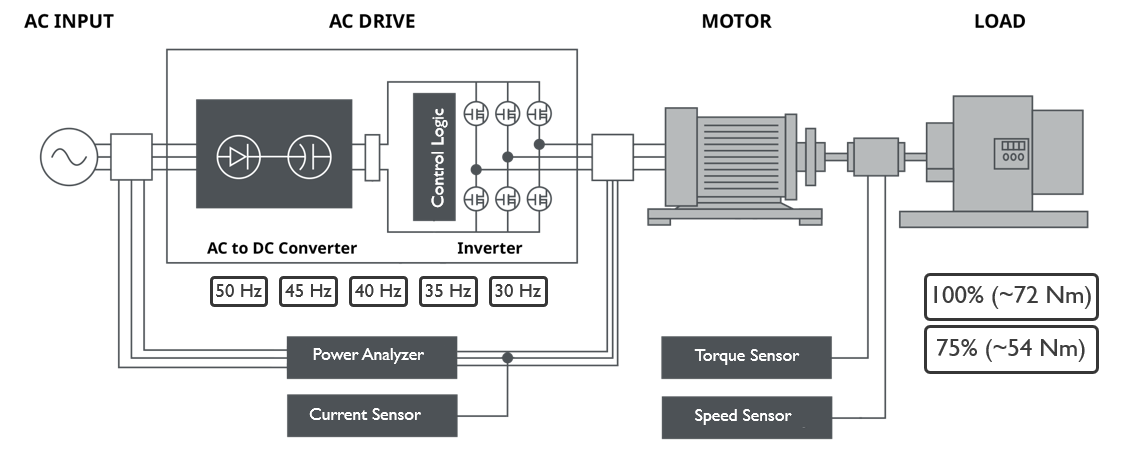
\includegraphics[width=400pt,keepaspectratio=true]{./fig/testsystem.PNG}
	% sekil3.eps: 0x0 pixel, 300dpi, 0.00x0.00 cm, bb=14 14 1155 740
	\caption{Schematic of test system.}	
	\label{schematic}
\end{figure}

Experimental studies were carried out at a rated load of 72 Nm and a frequency of 30, 35, 40, 45 and 50 Hz at 54 Nm, which is 75\% of the rated load, by applying the v/f control method over the VFD. Three motors produced in the same series on the same production line were taken and their data were collected in "healthy" condition under the mentioned conditions. For bearing failure, a fault was artificially created after hammering the drive-end bearing of one of the motors, while for stator failure, the insulation between the two turns in one phase of another motor was eroded. For the last motor, one of the bars in the rotor cage has been drilled for rotor failure. It should also be noted that studies conducted only for two cases in steady-state conditions for the motor as healthy and faulty.

\begin{table*}[h]
	{\setlength{\tabcolsep}{12pt}
		\caption{Brief information about the experimental conditions.}
		\begin{center}
			\vspace{-6mm}
			\begin{tabular}{ccc}
				\hline \\[-2.45ex] \hline \\[-2.1ex]
				Fault Type & Frequency ($Hz$) & Load $(N\cdot m)$ \\
				\hline \\[-1.8ex]
				Bearing & 30 & $\approx$ 72  \\
				Stator turn-turn & 35 & $\approx$ 54  \\
				Broken Rotor Bar & 40 &  \\
				& 45 &   \\
				& 50 &   \\
				\hline
			\end{tabular}
			\vspace{-6mm}
		\end{center}
		\label{Table3.3}}
\end{table*}

Another issue to be considered while collecting data is the amount of data required to see the effects of failure. In the experiments, the mechanical speed of the rotor varies between 857 and 1472 rpm in proportion to the reference control command applied. According to equation the given in \ref{data} \cite{shenfield2020novel}, approximately 200 data points are taken per revolution of the rotor shaft with 5 kHz sampling frequency and sampling time of 10 seconds, a window width of 50,000 data points, fault impacts expected to be easily captured.

\begin{equation}
	\textit{Number of Data Points} = \displaystyle \frac{60 \cdot \textit{Sampling Frequency (Hz)}}{\textit{Rotor's Mechanical Speed}}
	\label{data}
\end{equation}

In data analysis, studies were carried out in time and frequency domains. In the time domain, the stator supply currents are studied in raw (no pre-prosessing), while in the frequency domain, Welch's power spectral density estimation is applied to the current data. Current signals obtained in 1 second for healthy and faulty conditions under different speed and load scenarios, as well as 10 times zoomed, are shared in Figure \ref{bearing100} to Figure \ref{rotor75}. Looking at the plots, it is not possible to interpret whether the motor is faulty in the time domain or even if it is faulty, which fault has occurred.
\pagebreak
\begin{figure}[p]
	\centering
	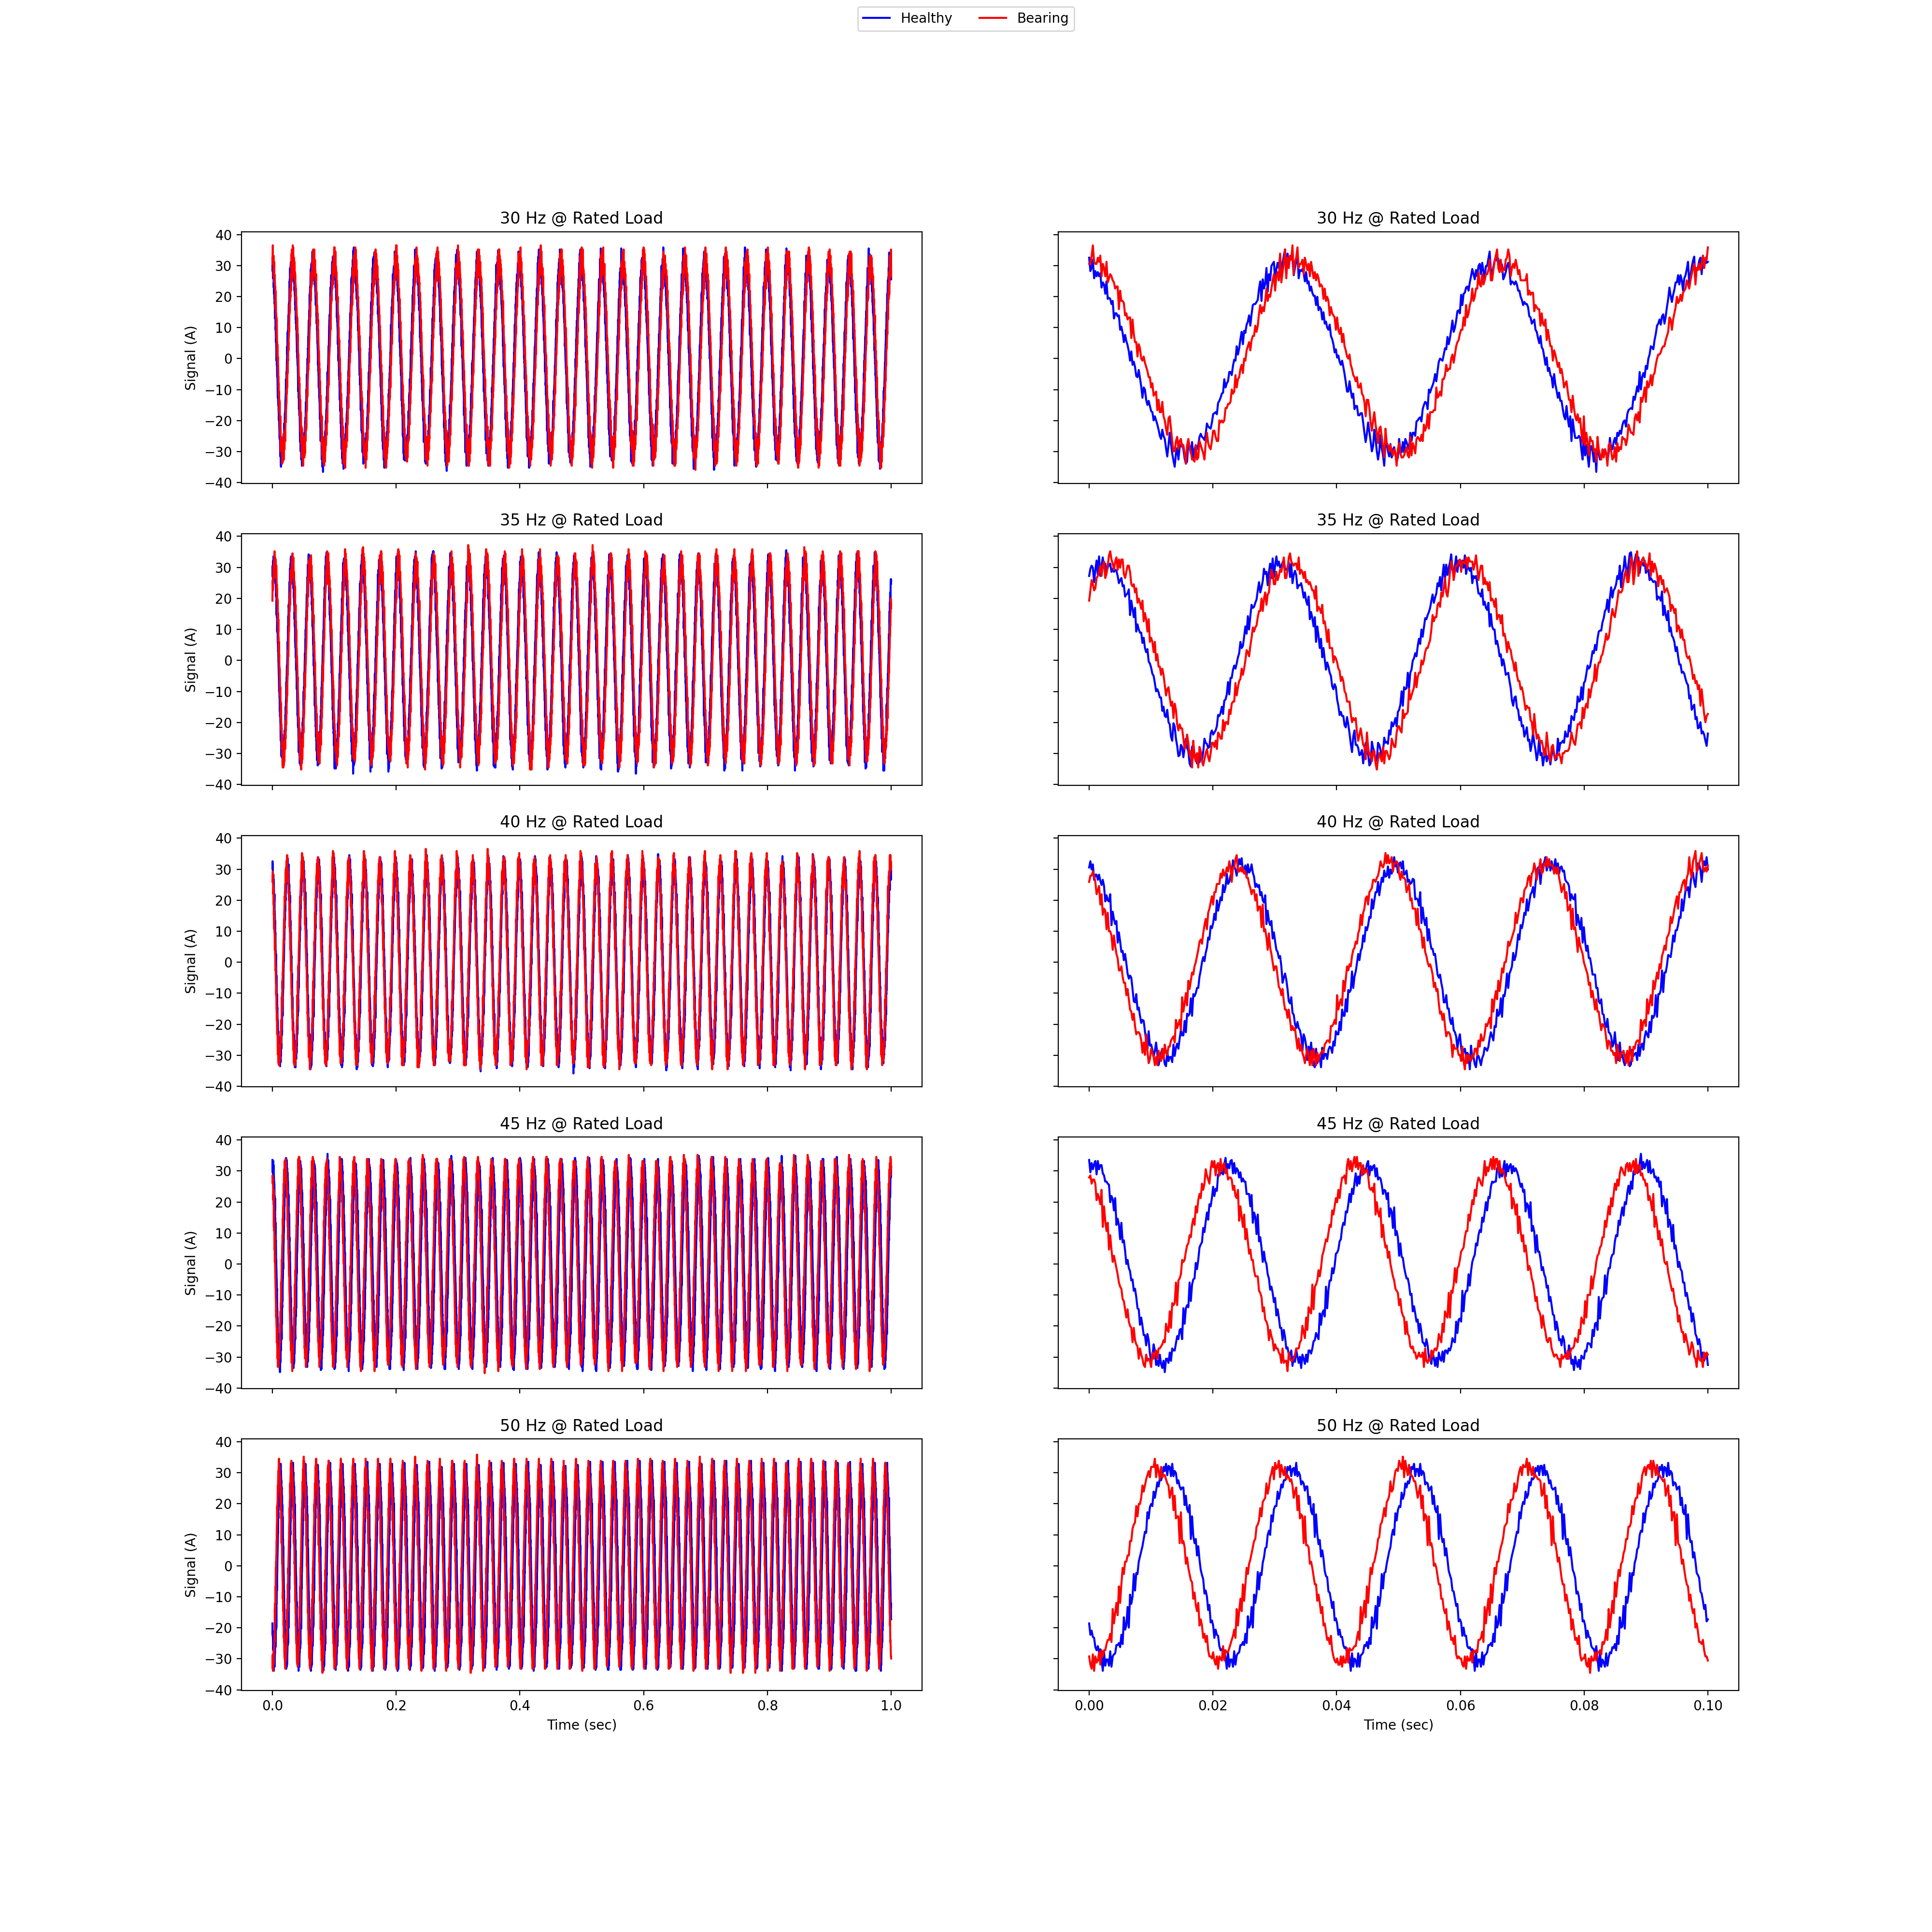
\includegraphics[width=0.75\paperwidth,keepaspectratio=true]{./fig/bearing_100.png}
	% sekil3.eps: 0x0 pixel, 300dpi, 0.00x0.00 cm, bb=14 14 1155 740
	\caption{An example of stator current signals of healthy and bearing-fault motor at rated load.}	
	\label{bearing100}
\end{figure}
\pagebreak
\begin{figure}[p]
	\centering
	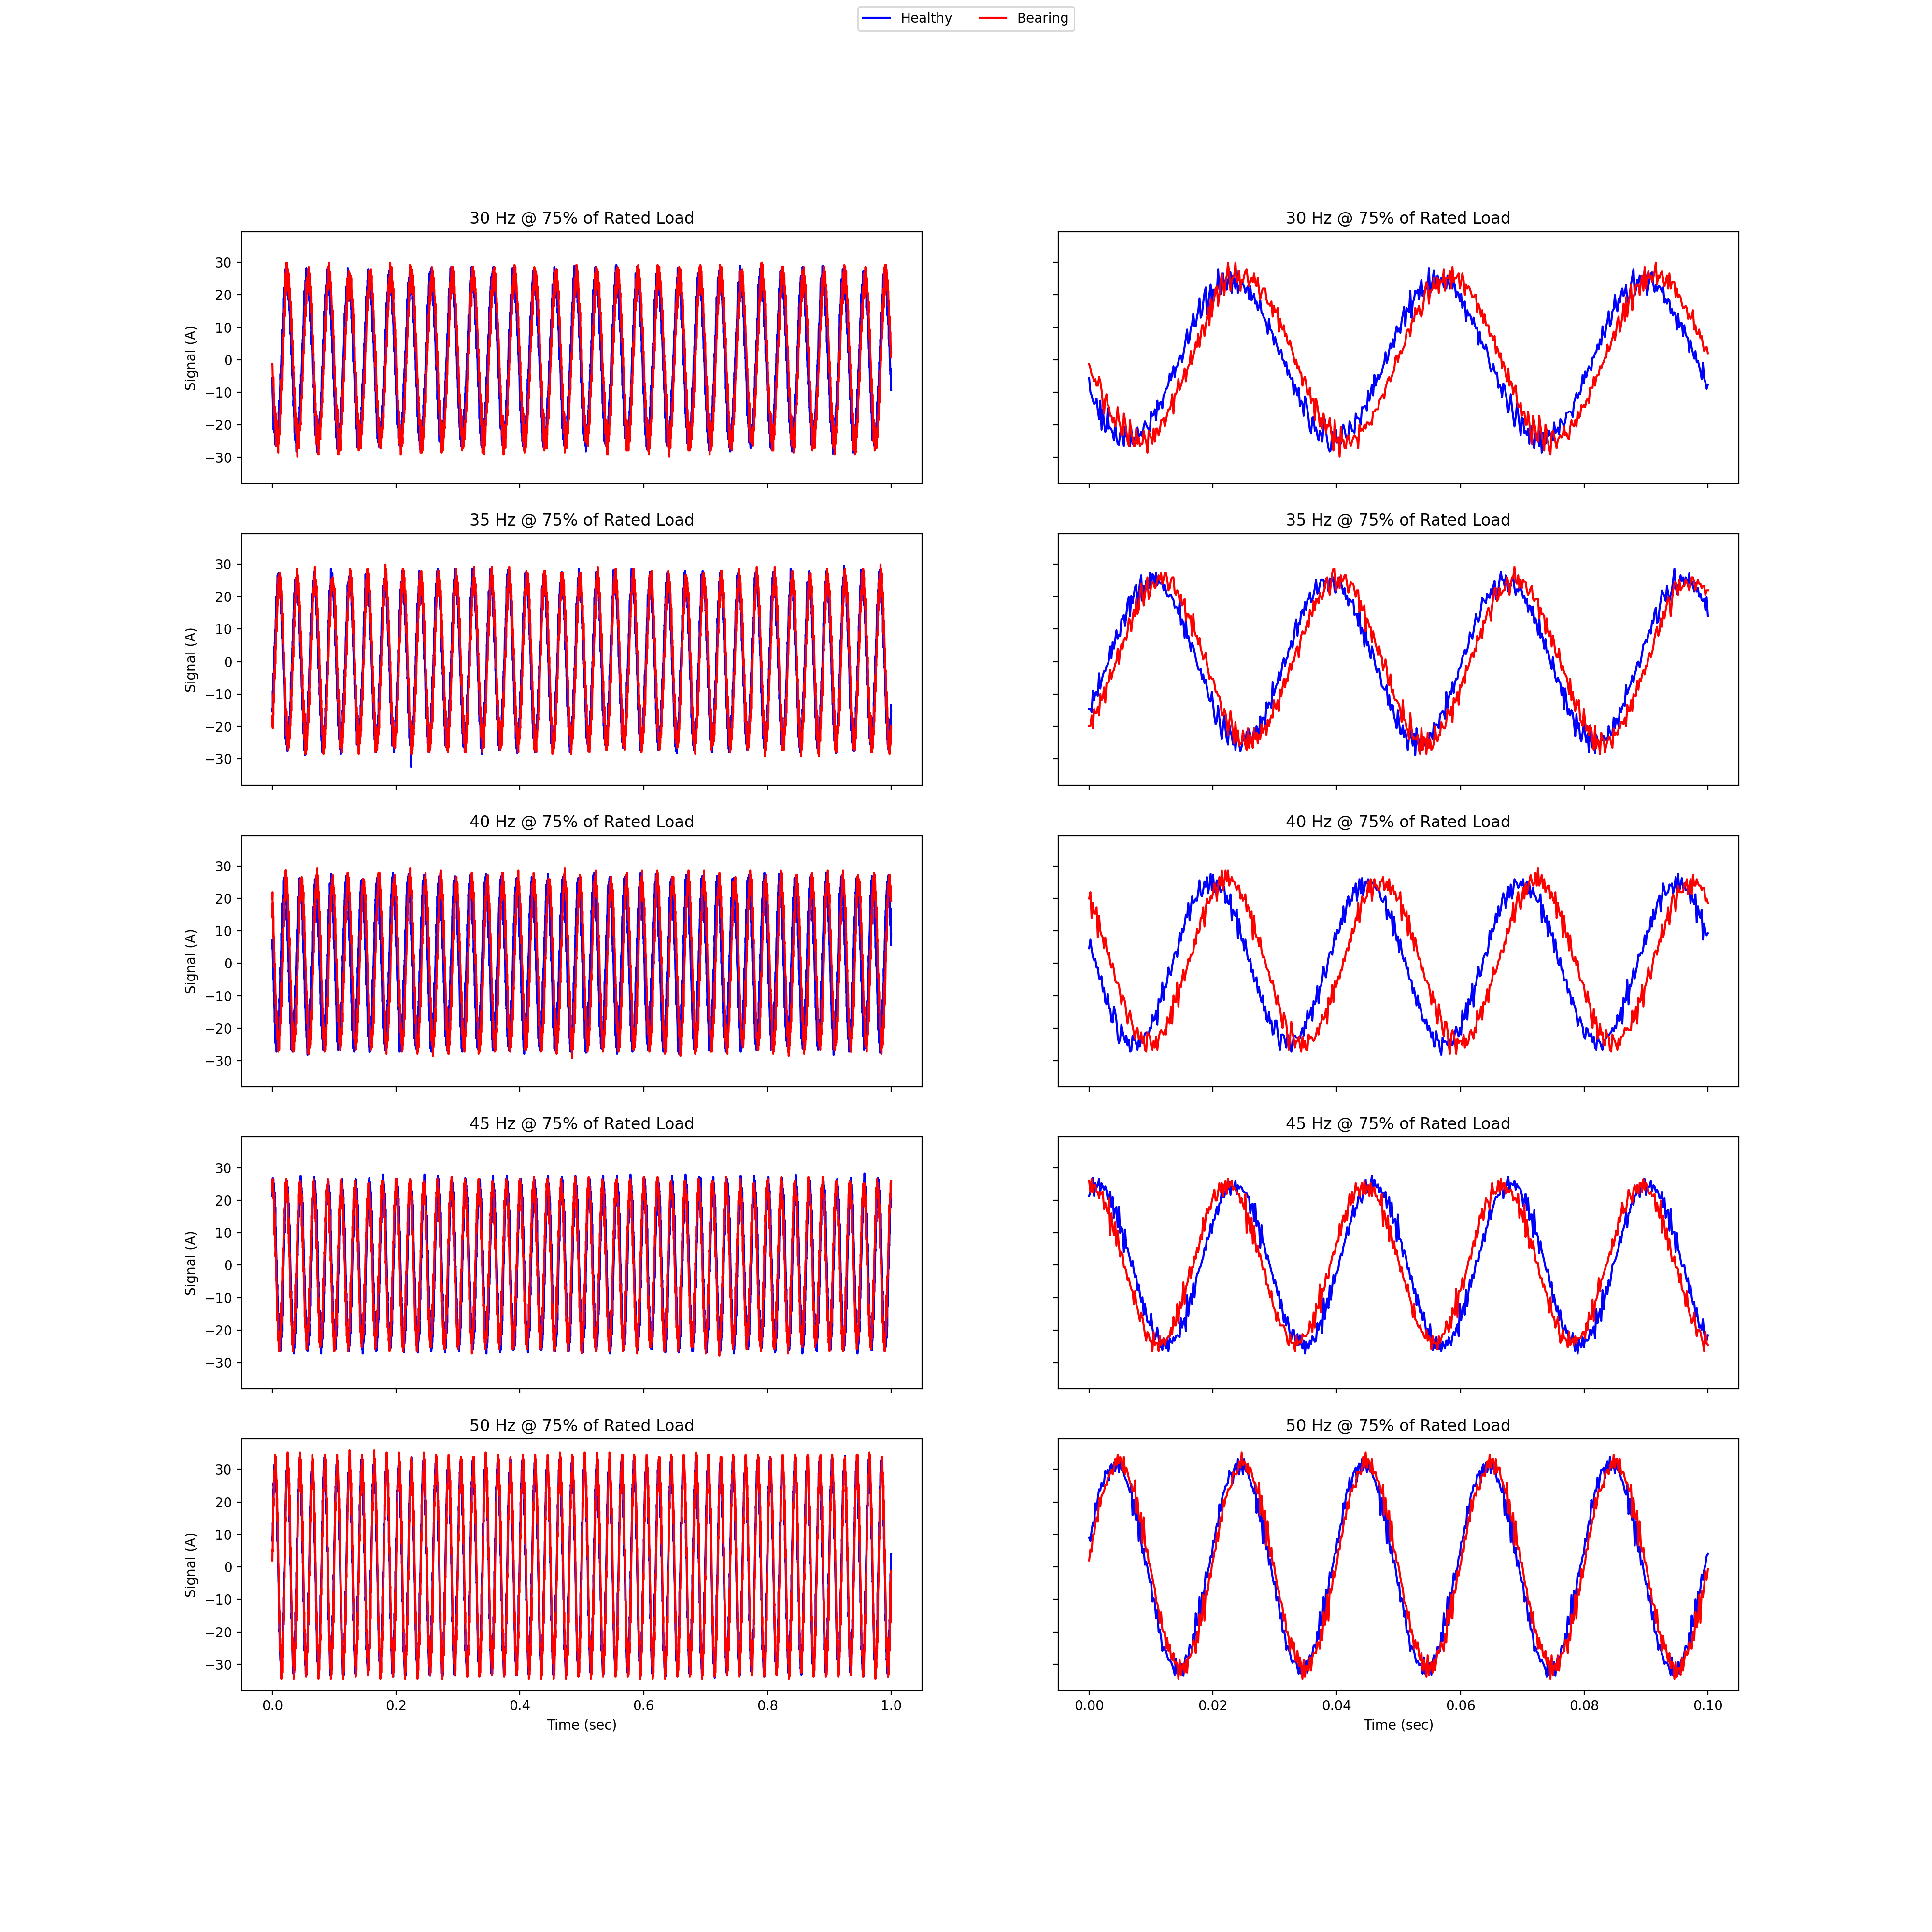
\includegraphics[width=0.75\paperwidth,keepaspectratio=true]{./fig/bearing_75.png}
	% sekil3.eps: 0x0 pixel, 300dpi, 0.00x0.00 cm, bb=14 14 1155 740
	\caption{An example of stator current signals of healthy and bearing-fault motor at $75\%$ of the rated load.}	
	\label{bearing75}
\end{figure}
\pagebreak
\begin{figure}[p]
	\centering
	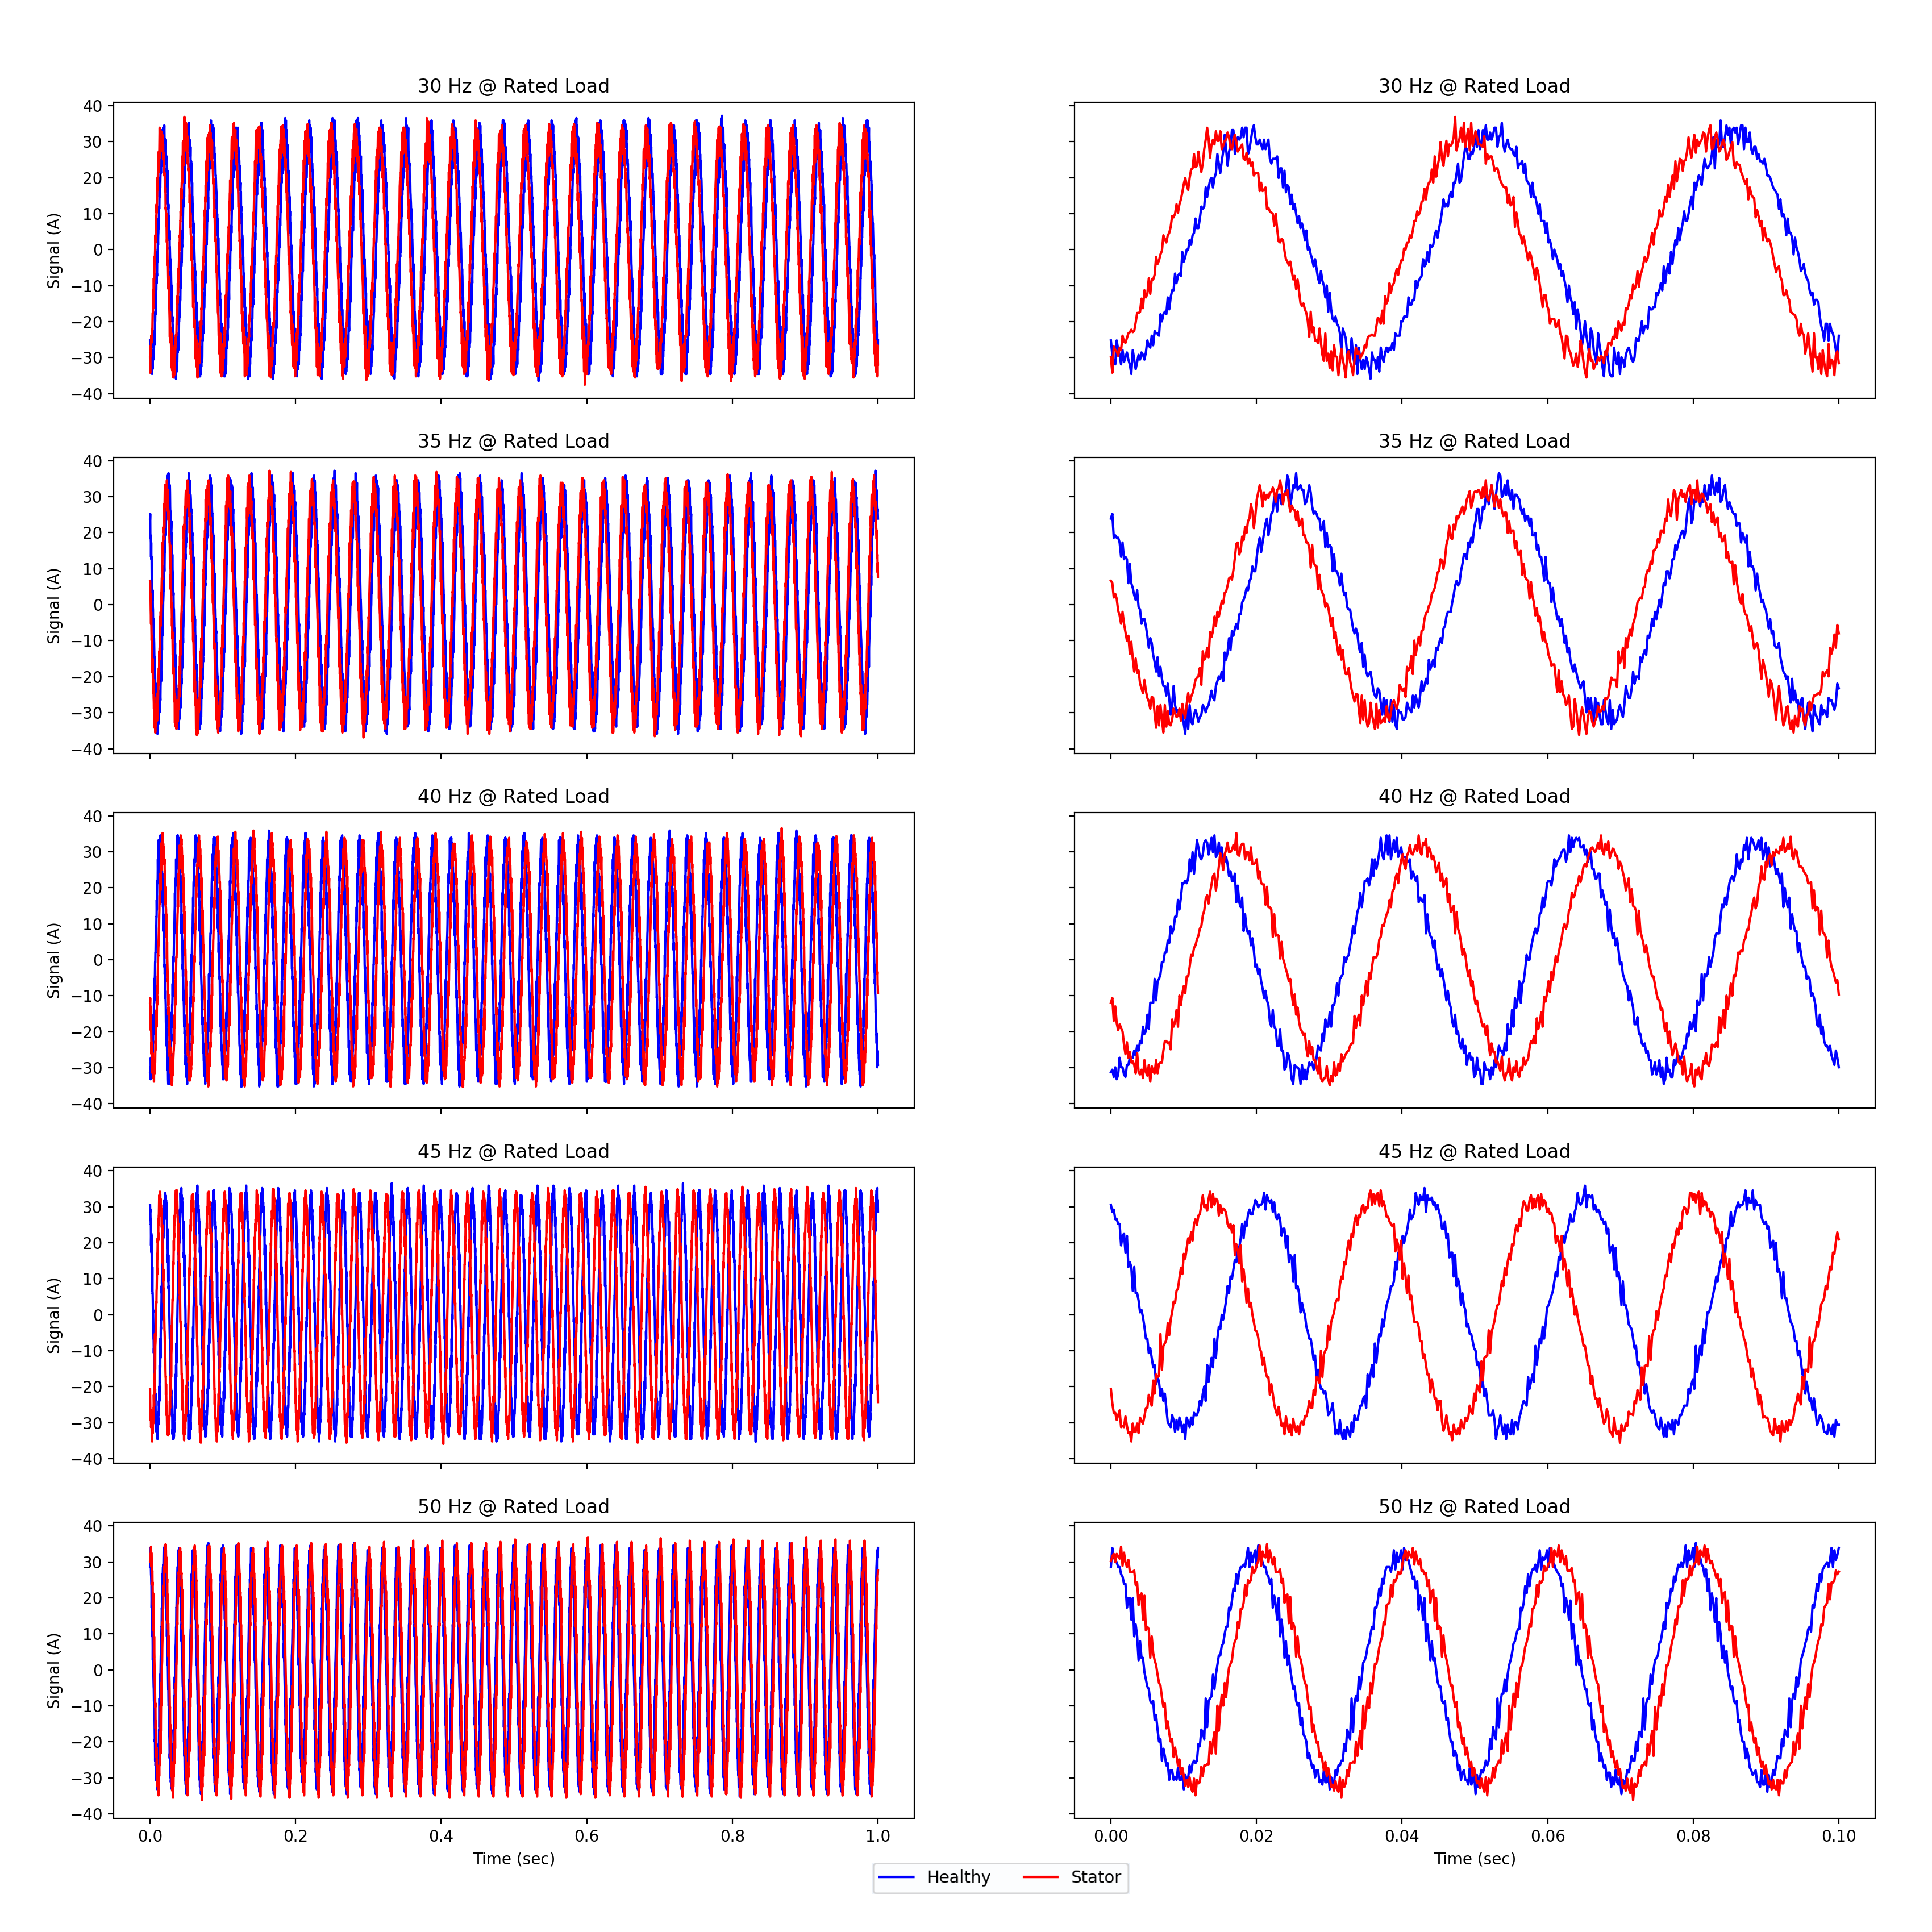
\includegraphics[width=0.75\paperwidth,keepaspectratio=true]{./fig/stator_100.png}
	% sekil3.eps: 0x0 pixel, 300dpi, 0.00x0.00 cm, bb=14 14 1155 740
	\caption{An example of stator current signals of healthy and stator inter-turn-fault motor at 75$\%$ of the rated load.}	
	\label{stator100}
\end{figure}
\pagebreak
\begin{figure}[p]
	\centering
	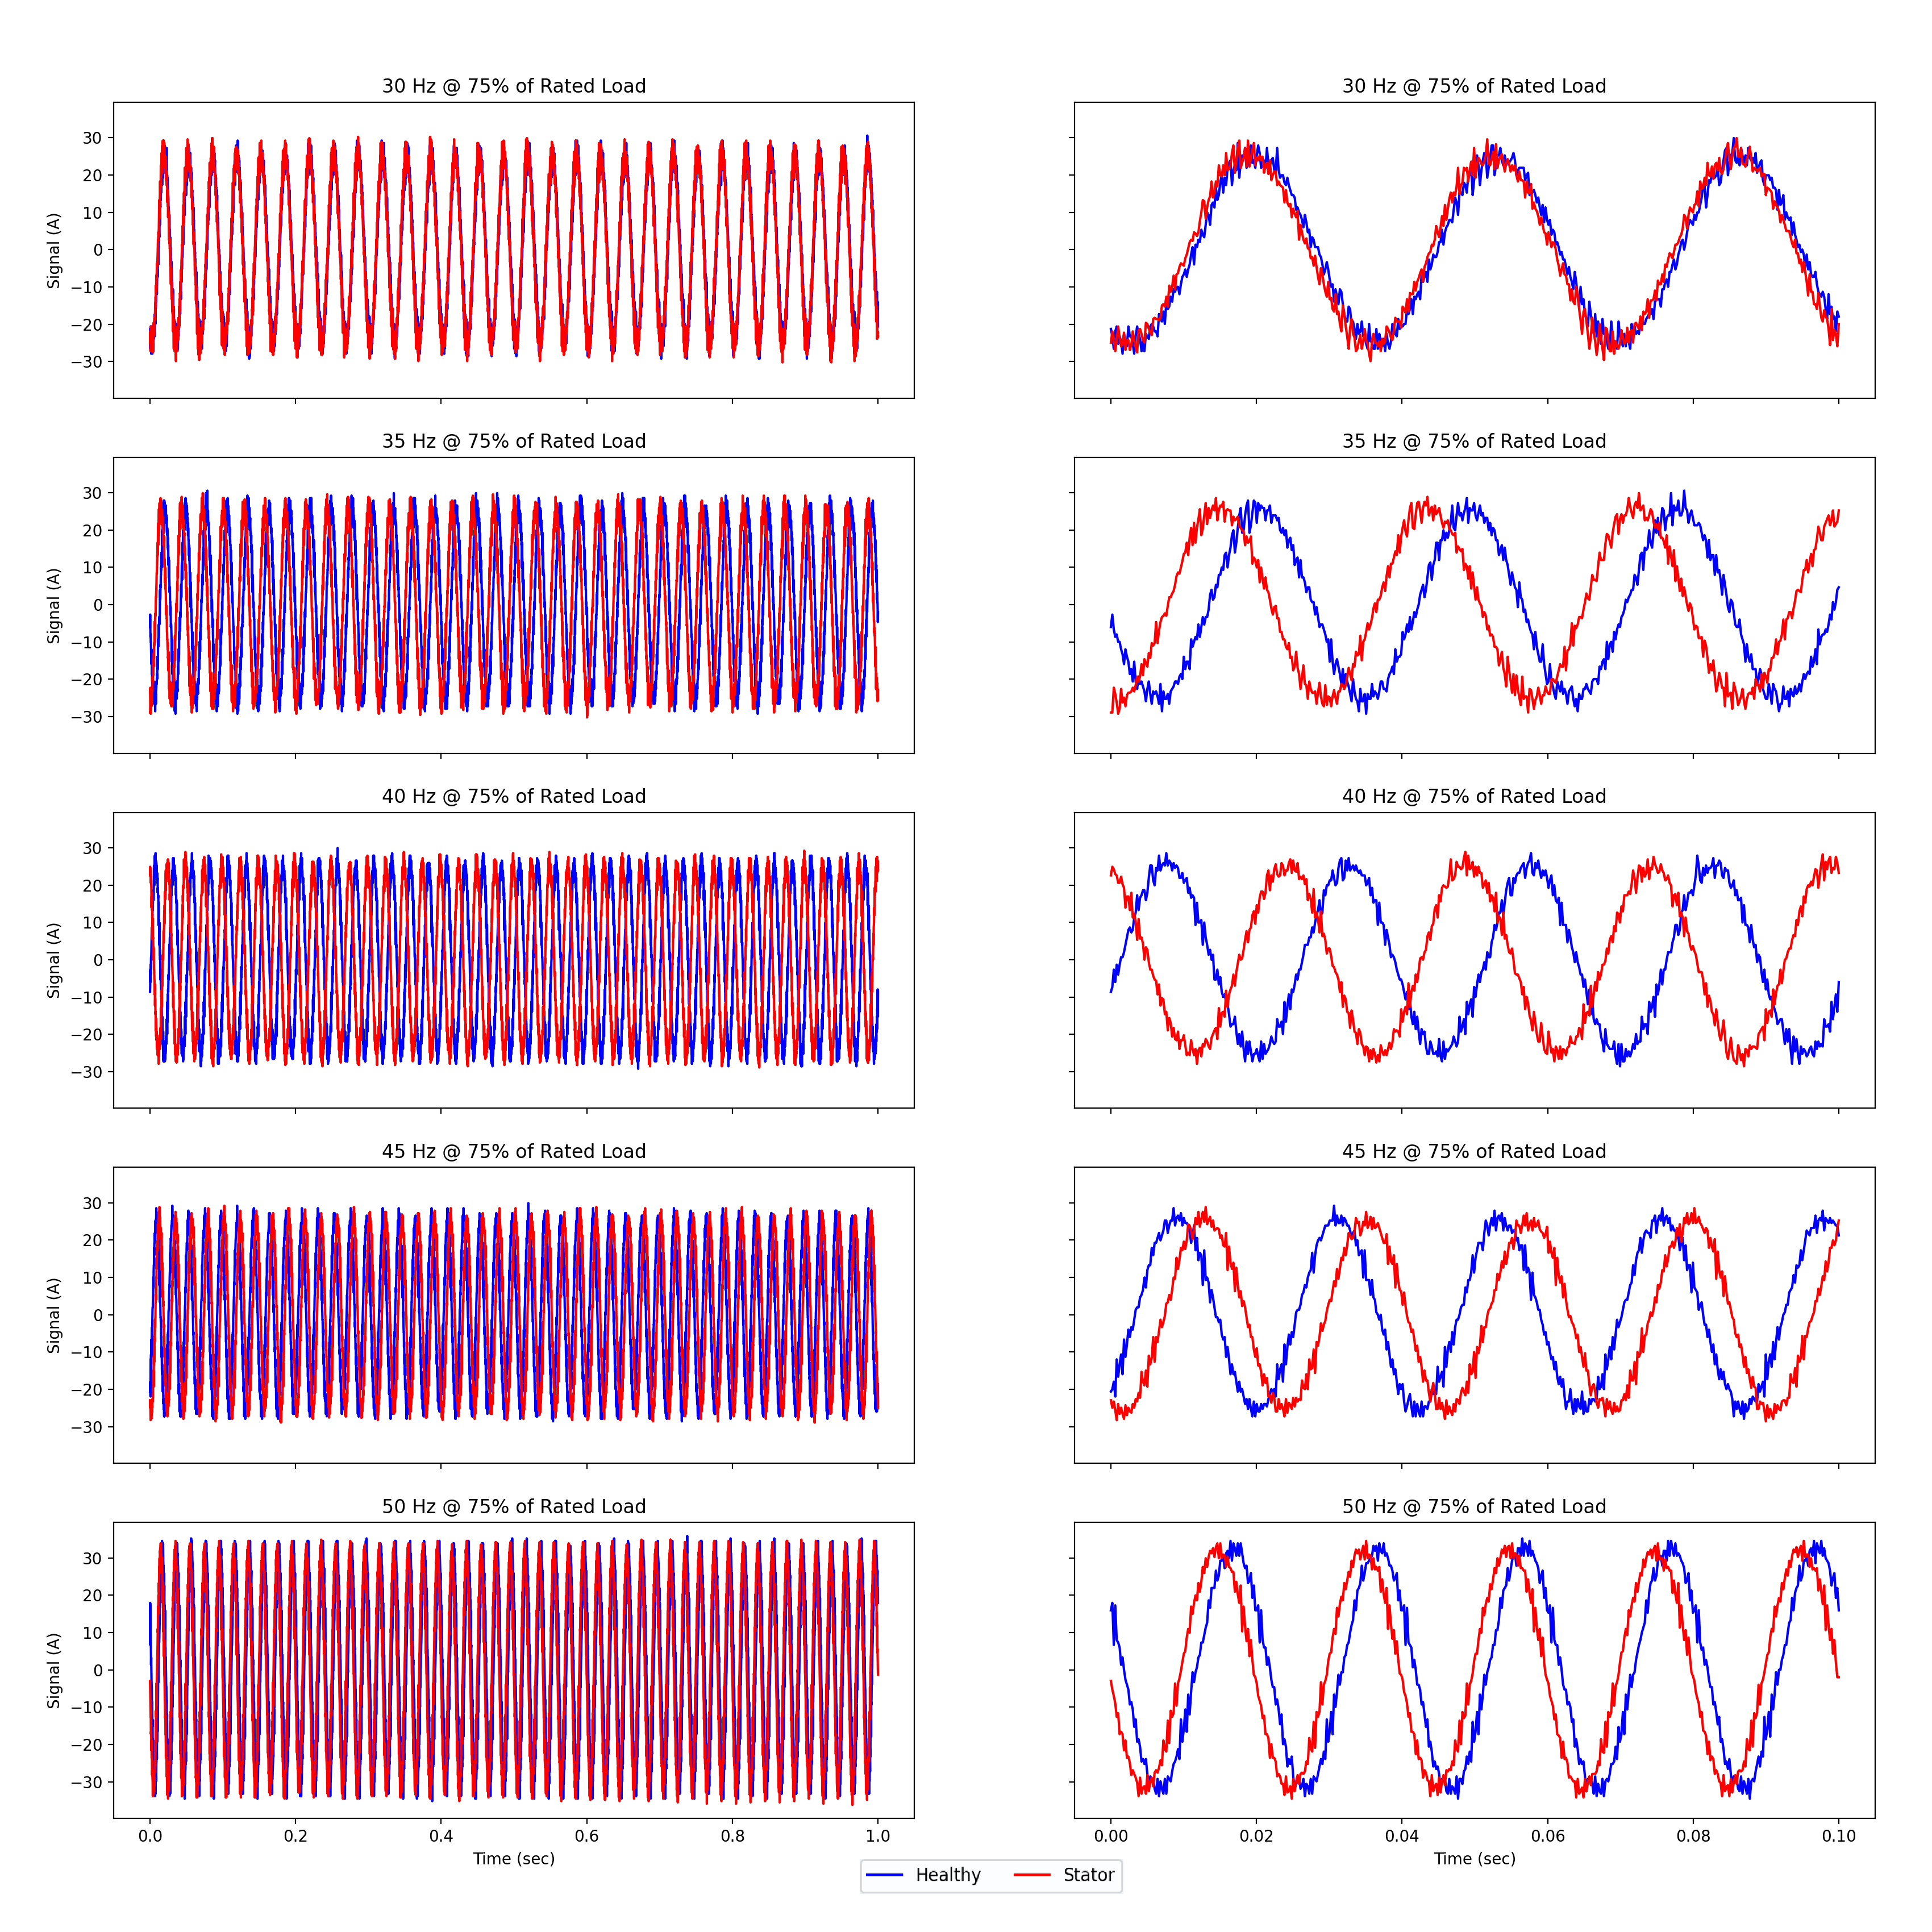
\includegraphics[width=0.75\paperwidth,keepaspectratio=true]{./fig/stator_75.png}
	% sekil3.eps: 0x0 pixel, 300dpi, 0.00x0.00 cm, bb=14 14 1155 740
	\caption{An example of stator current signals of healthy and stator inter-turn-fault motor at 75$\%$ of the rated load.}	
	\label{stator75}
\end{figure}
\pagebreak
\begin{figure}[p]
	\centering
	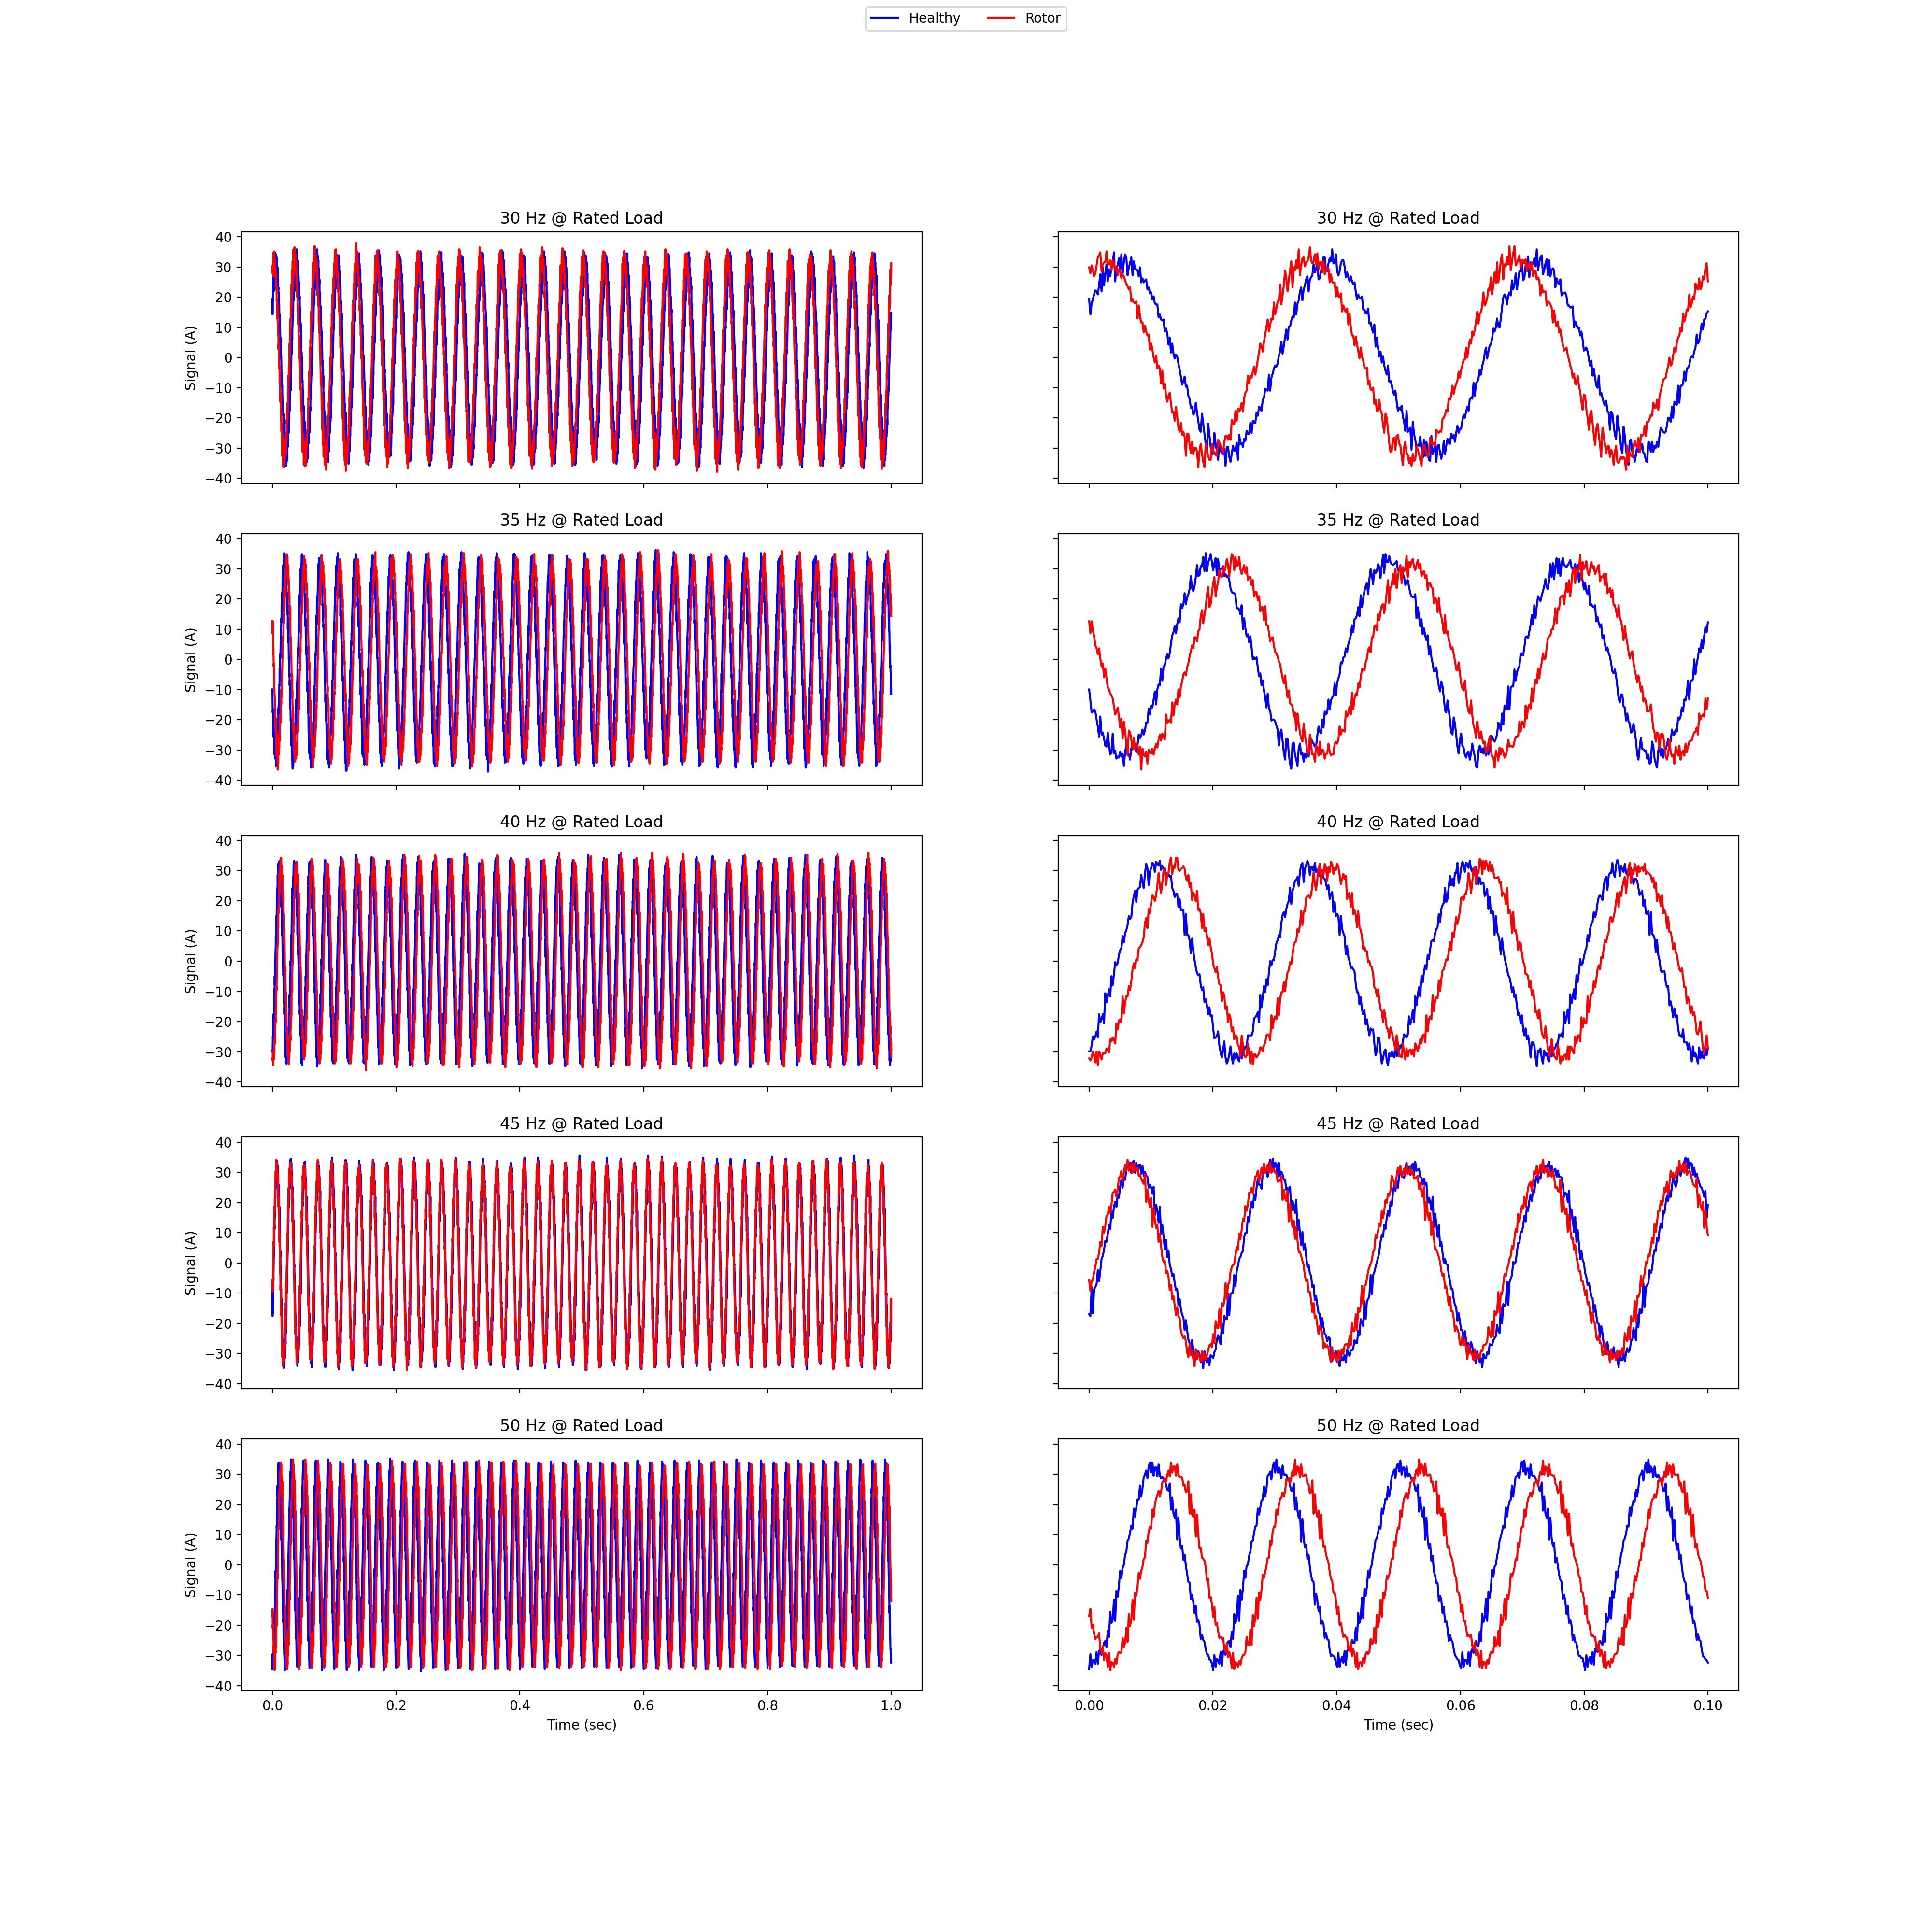
\includegraphics[width=0.75\paperwidth,keepaspectratio=true]{./fig/rotor_100.png}
	% sekil3.eps: 0x0 pixel, 300dpi, 0.00x0.00 cm, bb=14 14 1155 740
	\caption{An example of stator current signals of healthy and broken rotor bar-fault motor at 75$\%$ of the rated load.}	
	\label{rotor100}
\end{figure}
\pagebreak
\begin{figure}[p]
	\centering
	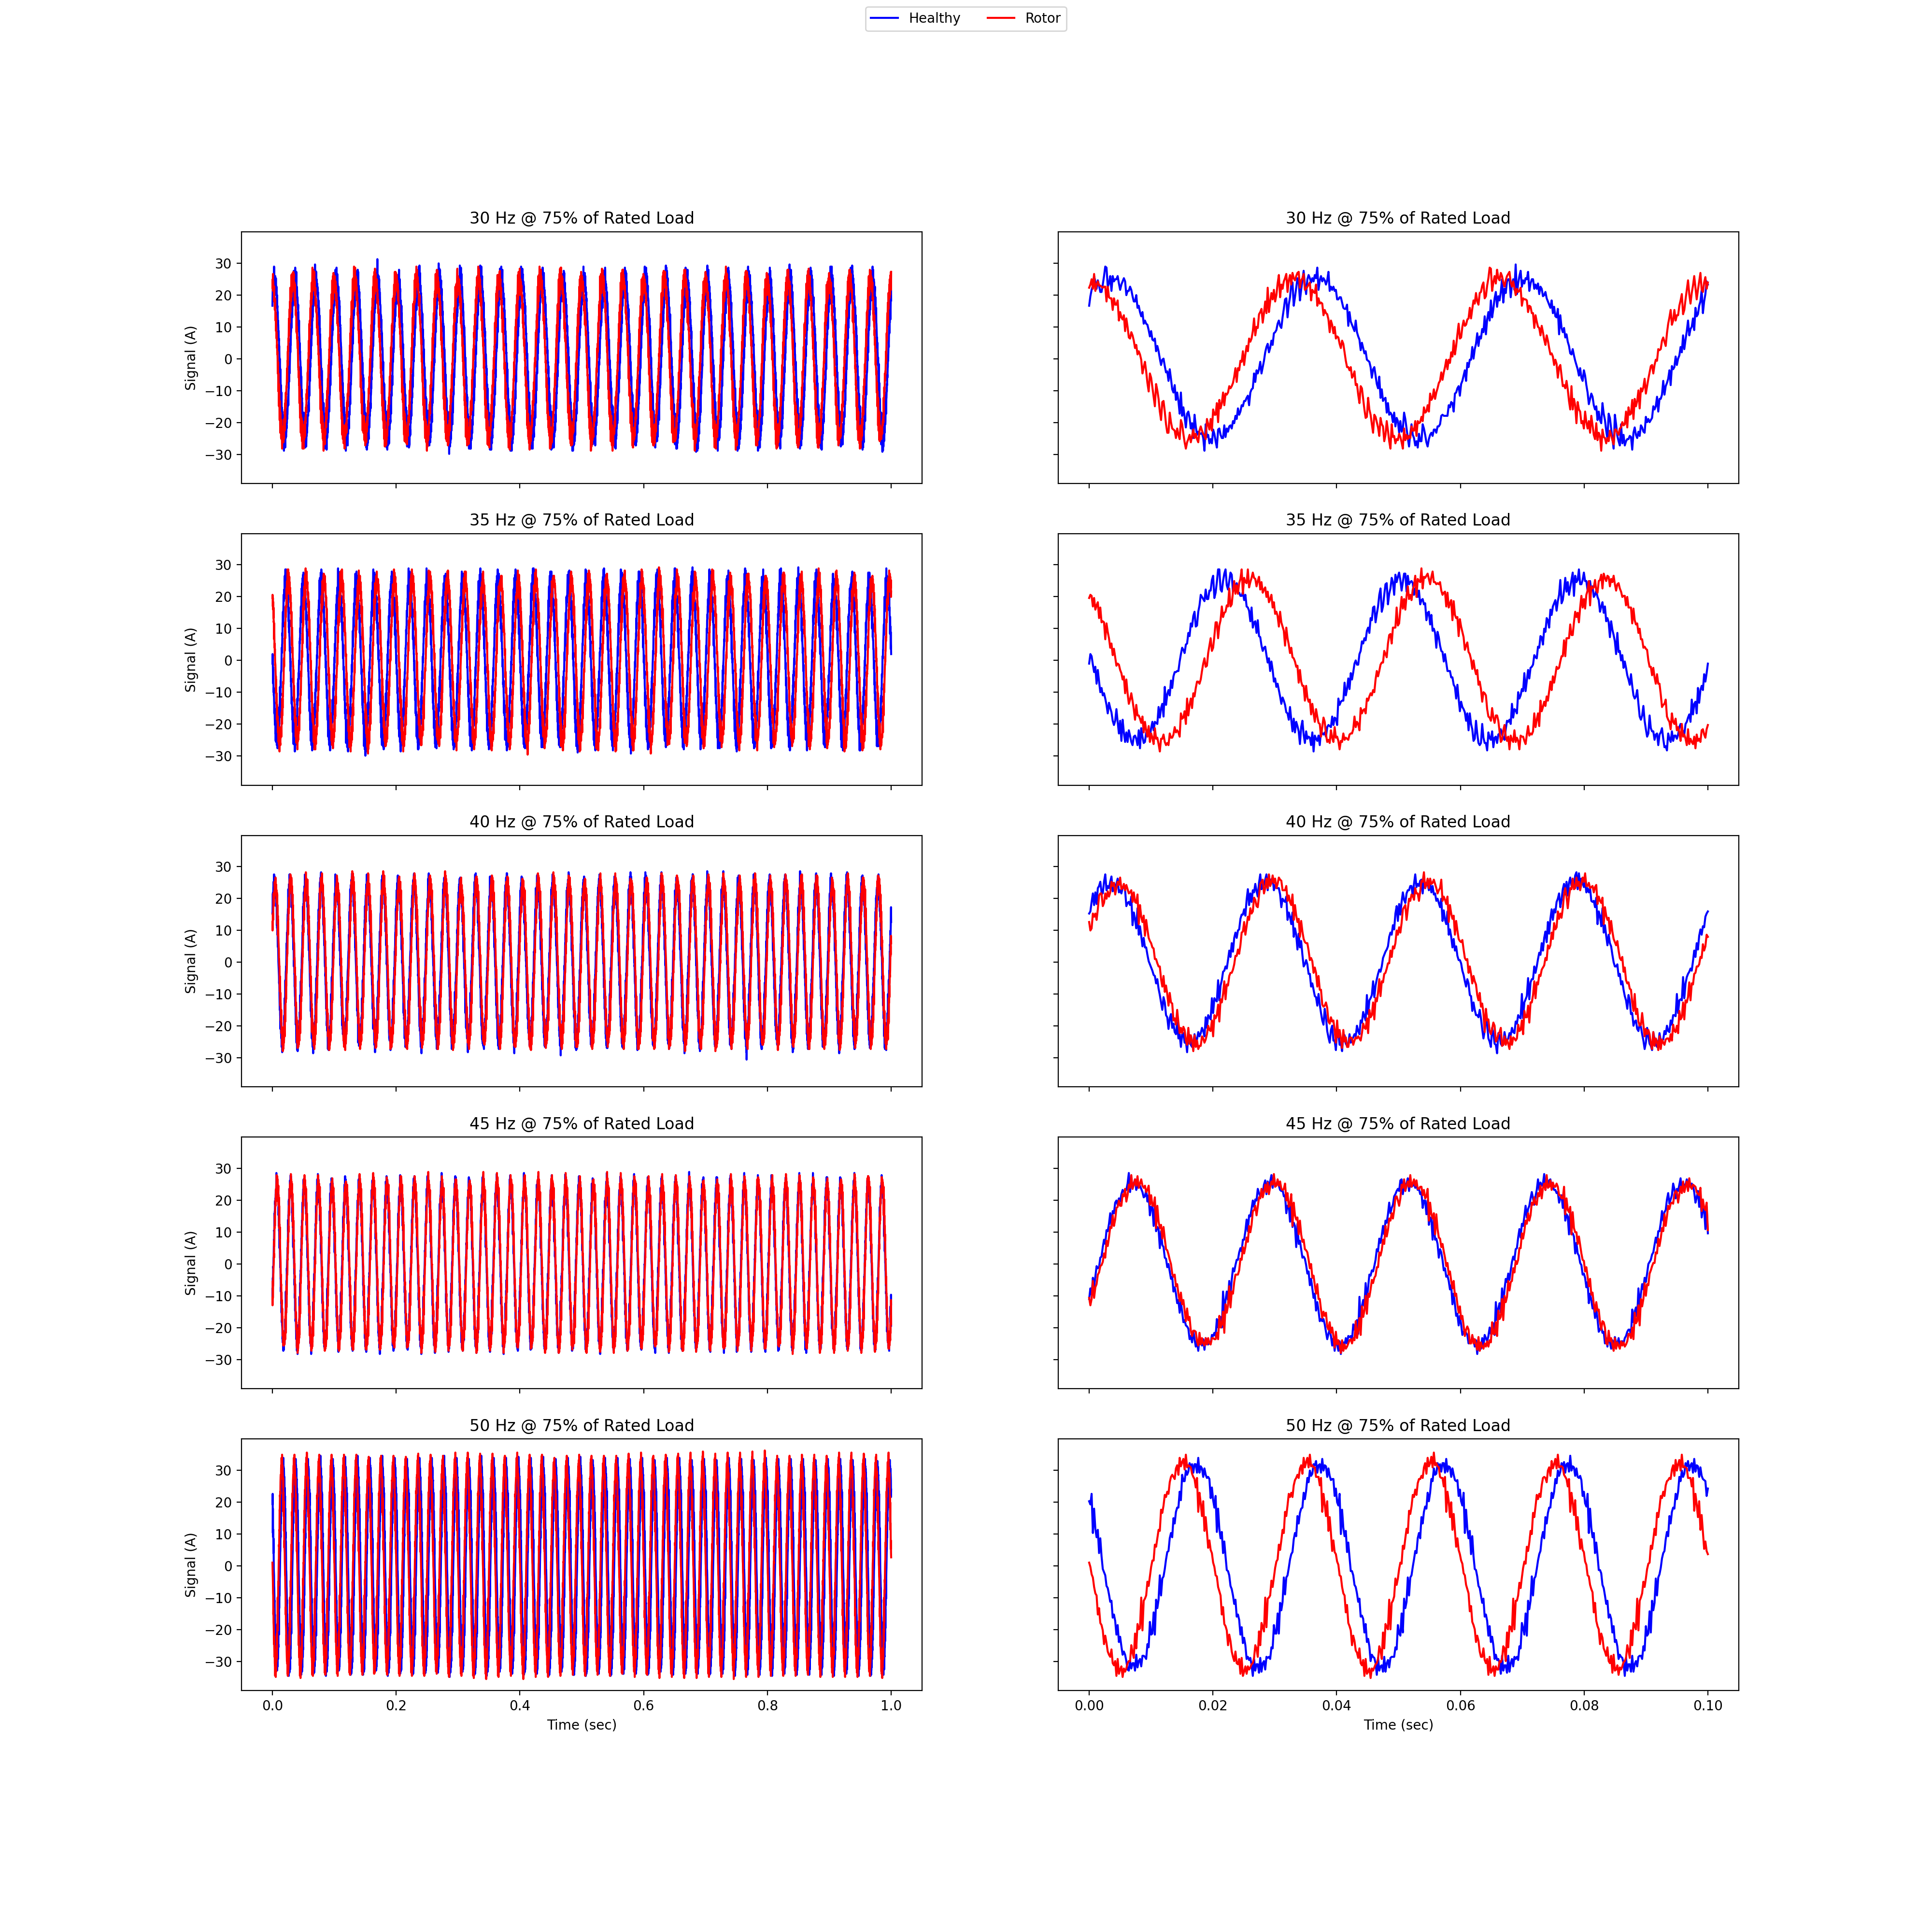
\includegraphics[width=0.75\paperwidth,keepaspectratio=true]{./fig/rotor_75.png}
	% sekil3.eps: 0x0 pixel, 300dpi, 0.00x0.00 cm, bb=14 14 1155 740
	\caption{An example of stator current signals of healthy and broken rotor bar-fault motor at 75$\%$ of the rated load.}	
	\label{rotor75}
\end{figure}
\pagebreak
\clearpage
In addition, Figures \ref{psdbearing100} to \ref{psdrotor75} demonstrate Welch's PSD estimation applied to healthy and faulty conditions of stator currents. Looking at the PSD graphs, there are visible differences between the faulty states and the healthy states, as well as the variation created by different faults at certain frequencies.

\begin{table*}[h]
	{\setlength{\tabcolsep}{12pt}
		\caption{Input parameters for estimating Welch's PSD.}
		\begin{center}
			\vspace{-6mm}
			\begin{tabular}{cc}
				\hline \\[-2.45ex] \hline \\[-2.1ex]
				Parameter & Value  \\
				\hline \\[-1.8ex]
				Window Type & Hamming    \\
				Overlap (\%) & 50 \\
				Number of DFT Points & 50000  \\
				Sample Rate & 5000    \\
				\hline
			\end{tabular}
			\vspace{-6mm}
		\end{center}
		\label{Table3.4}}
\end{table*}
\pagebreak

\begin{figure}[p]
	\centering
	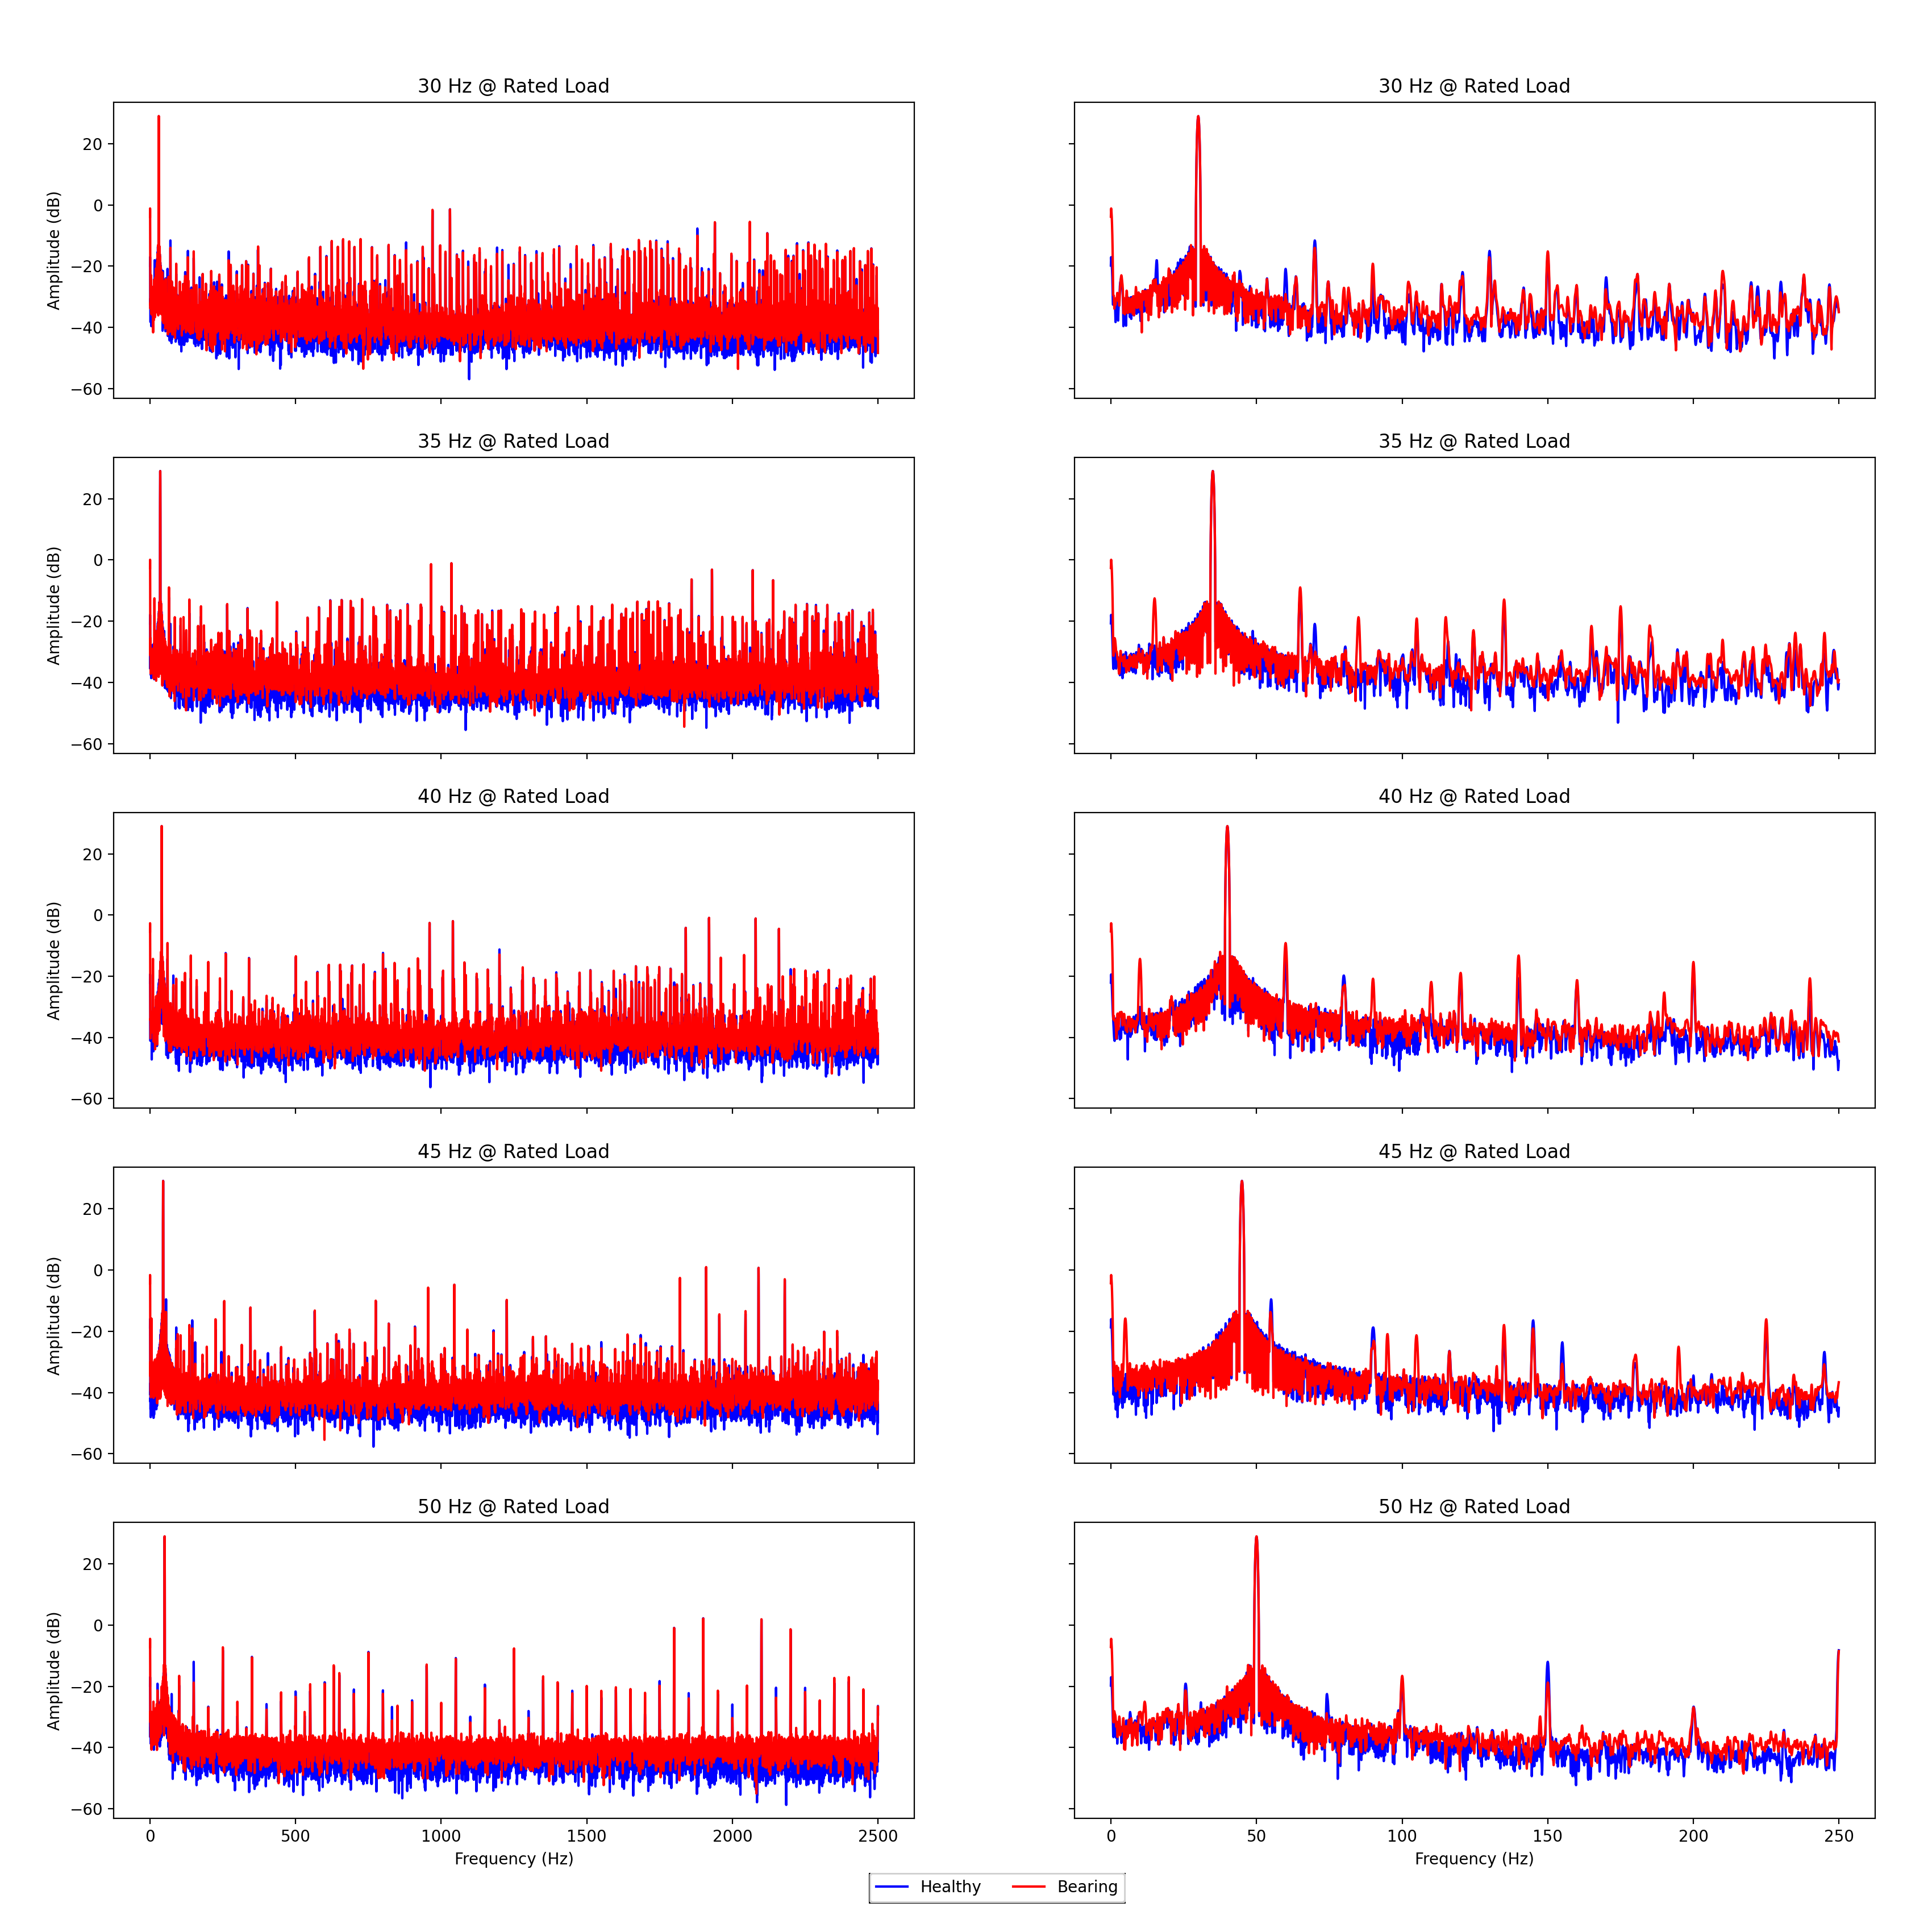
\includegraphics[width=0.75\paperwidth,keepaspectratio=true]{./fig/psdbearing_100.png}
	% sekil3.eps: 0x0 pixel, 300dpi, 0.00x0.00 cm, bb=14 14 1155 740
	\caption{Welch's PSD estimations of healthy and bearing-fault motor at rated load.}	
	\label{psdbearing100}
\end{figure}
\pagebreak
\begin{figure}[p]
	\centering
	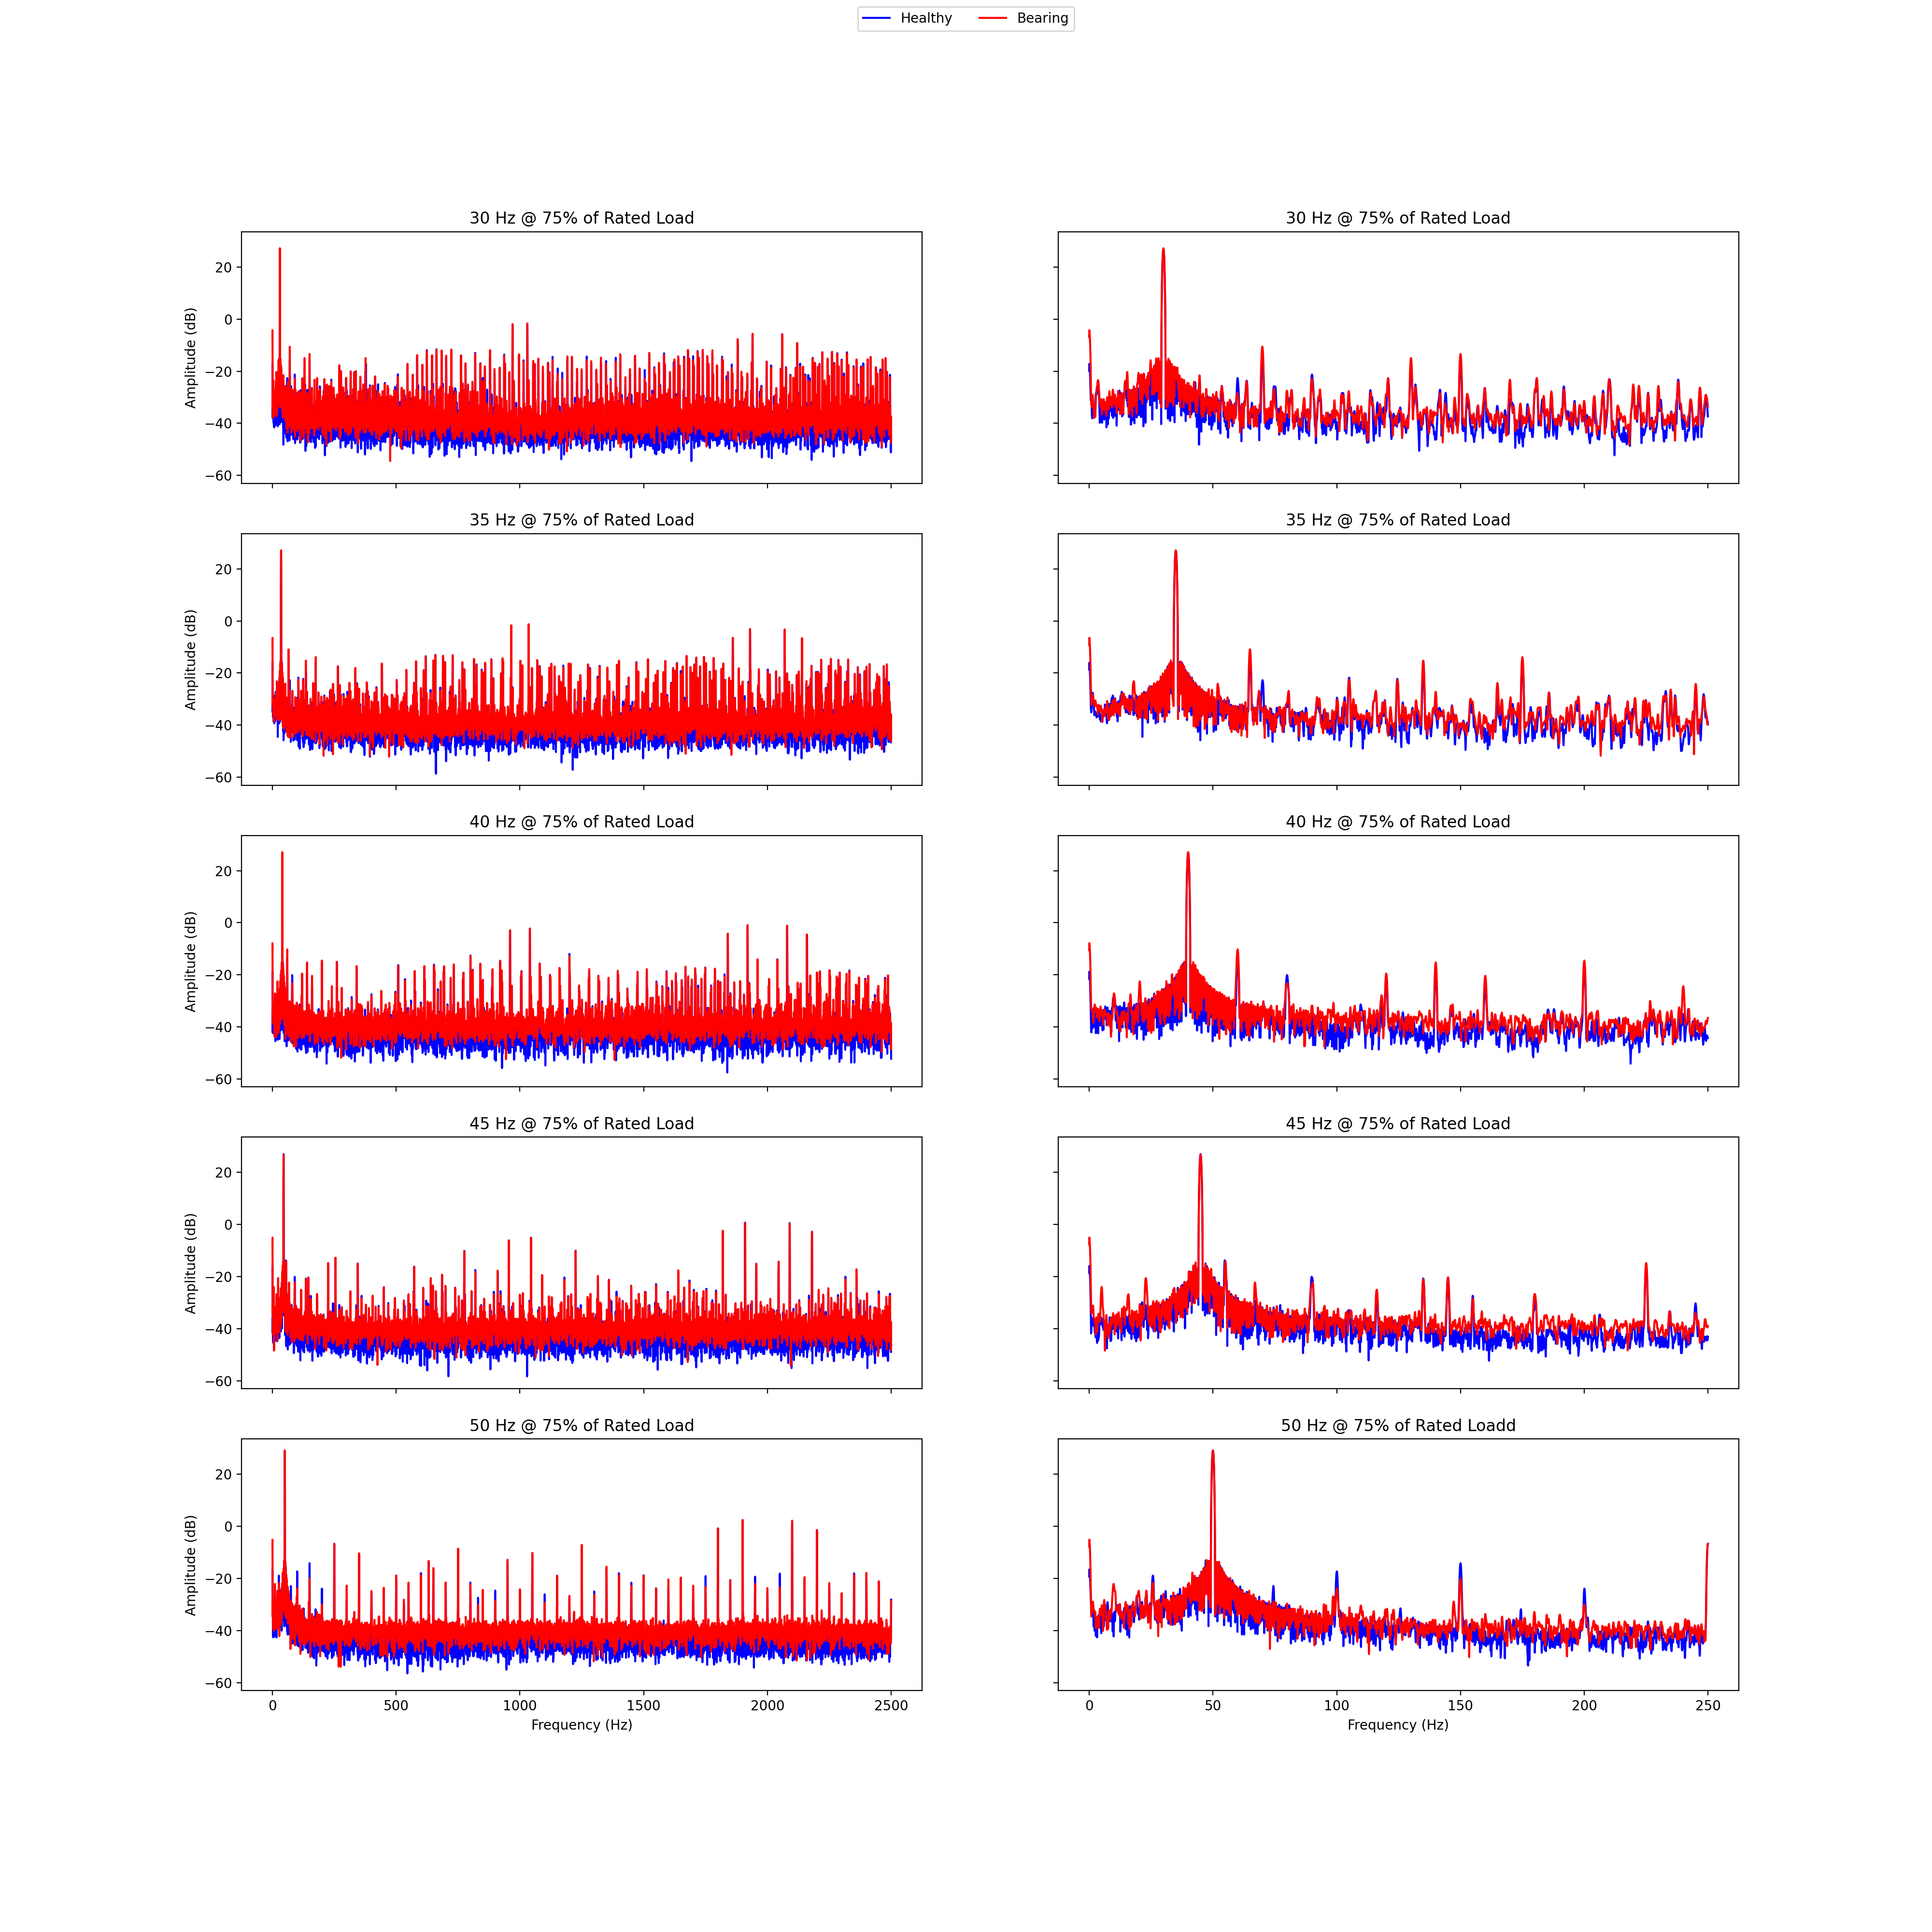
\includegraphics[width=0.75\paperwidth,keepaspectratio=true]{./fig/psdbearing_75.png}
	% sekil3.eps: 0x0 pixel, 300dpi, 0.00x0.00 cm, bb=14 14 1155 740
	\caption{Welch's PSD estimations of healthy and bearing-fault motor at $75\%$ of the rated load.}	
	\label{psdbearing75}
\end{figure}
\pagebreak
\begin{figure}[p]
	\centering
	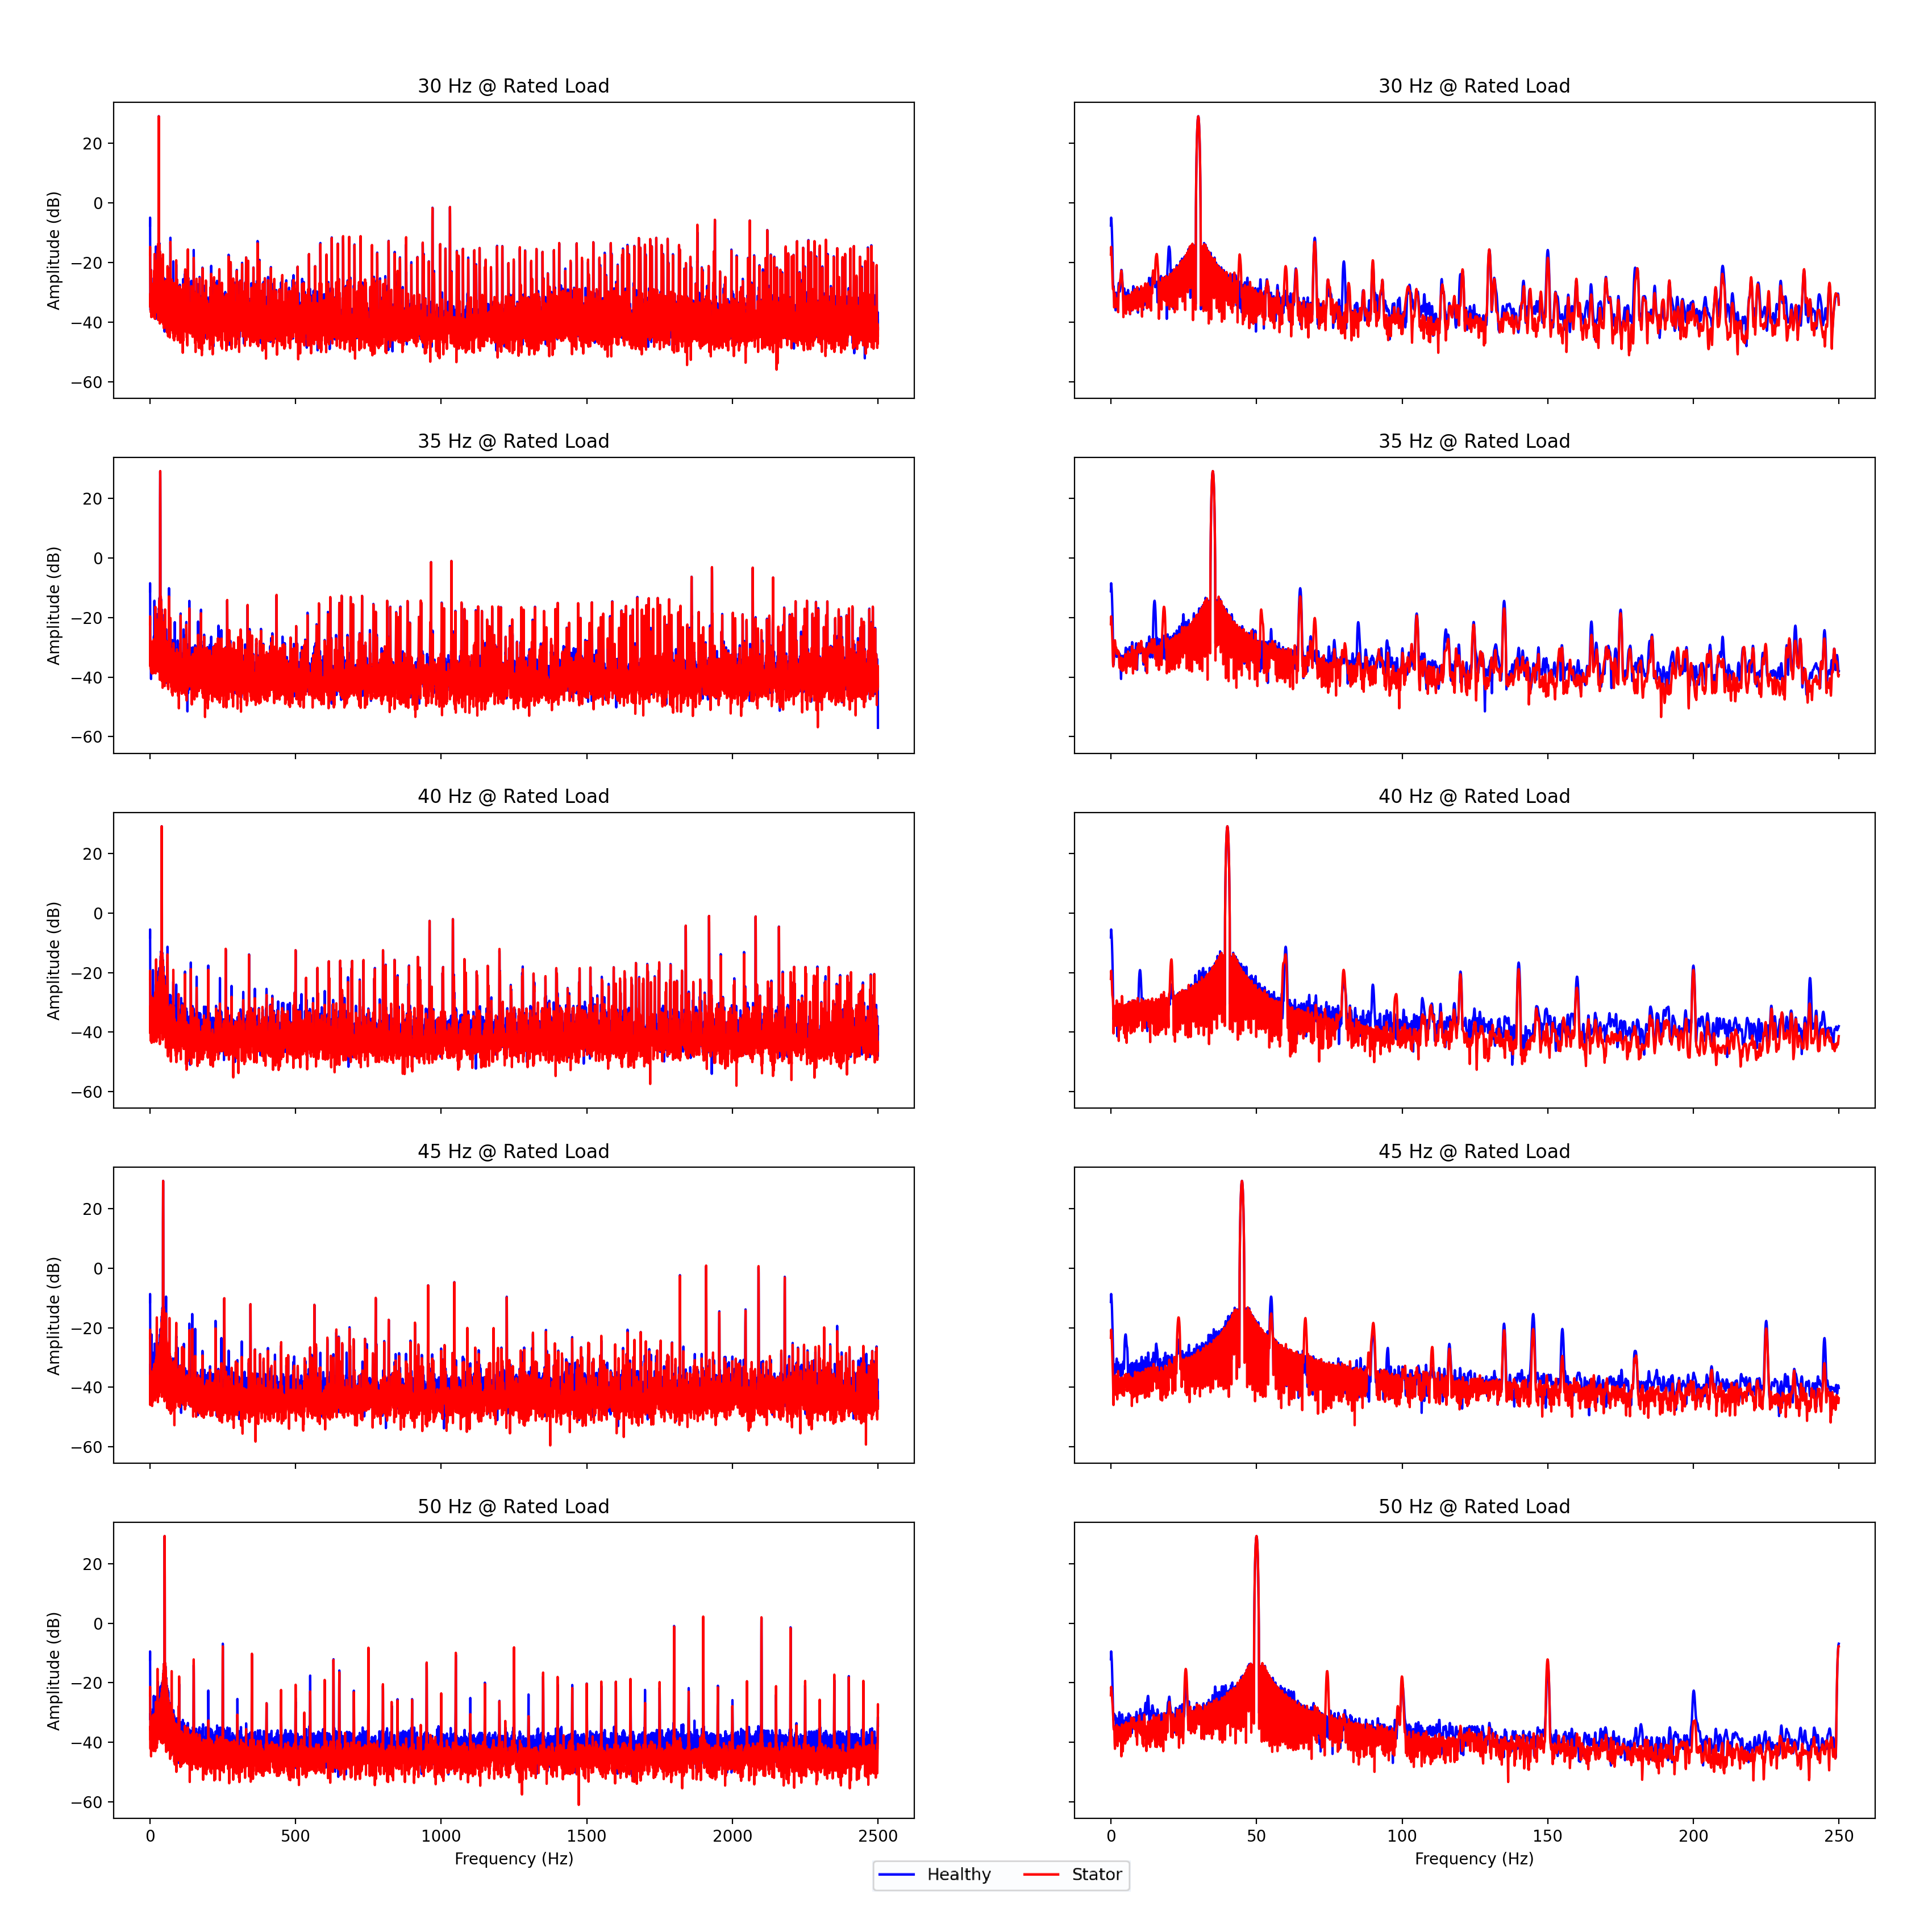
\includegraphics[width=0.75\paperwidth,keepaspectratio=true]{./fig/psdstator_100.png}
	% sekil3.eps: 0x0 pixel, 300dpi, 0.00x0.00 cm, bb=14 14 1155 740
	\caption{Welch's PSD estimations of healthy and stator inter-turn-fault motor at 75$\%$ of the rated load.}	
	\label{psdstator100}
\end{figure}
\pagebreak
\begin{figure}[p]
	\centering
	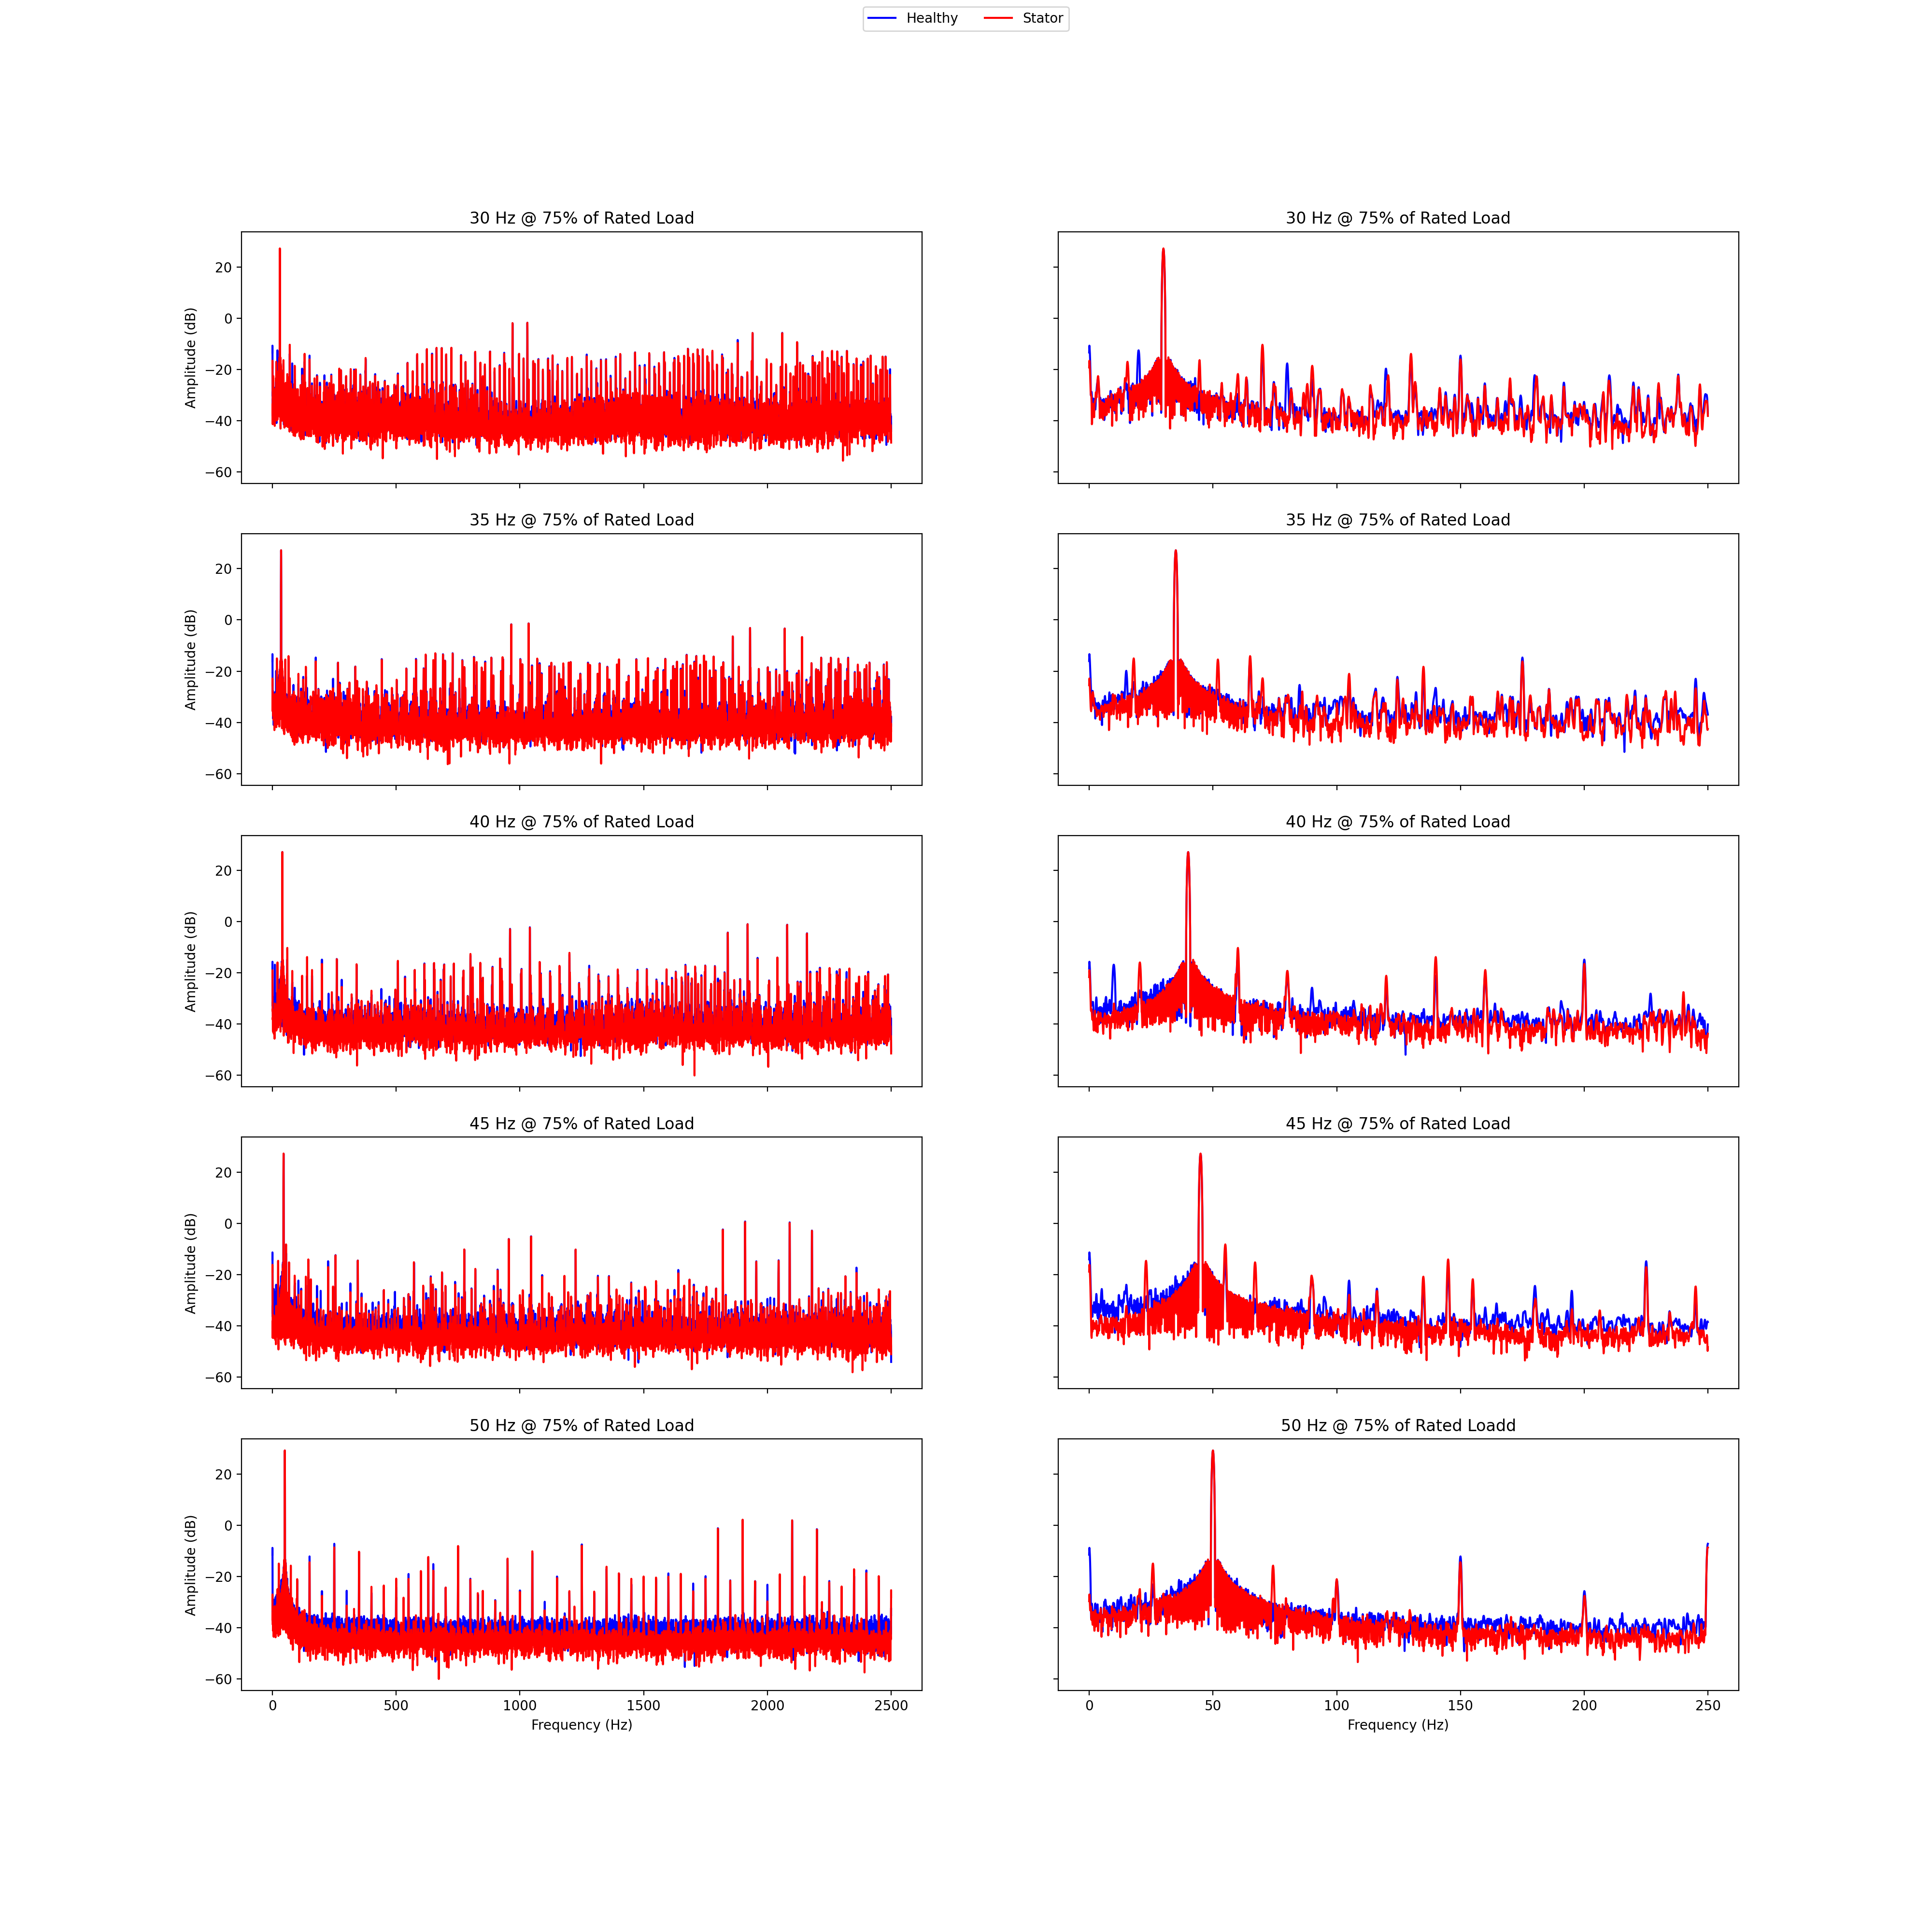
\includegraphics[width=0.75\paperwidth,keepaspectratio=true]{./fig/psdstator_75.png}
	% sekil3.eps: 0x0 pixel, 300dpi, 0.00x0.00 cm, bb=14 14 1155 740
	\caption{Welch's PSD estimations of healthy and stator inter-turn-fault motor at 75$\%$ of the rated load.}	
	\label{psdstator75}
\end{figure}
\pagebreak
\begin{figure}[p]
	\centering
	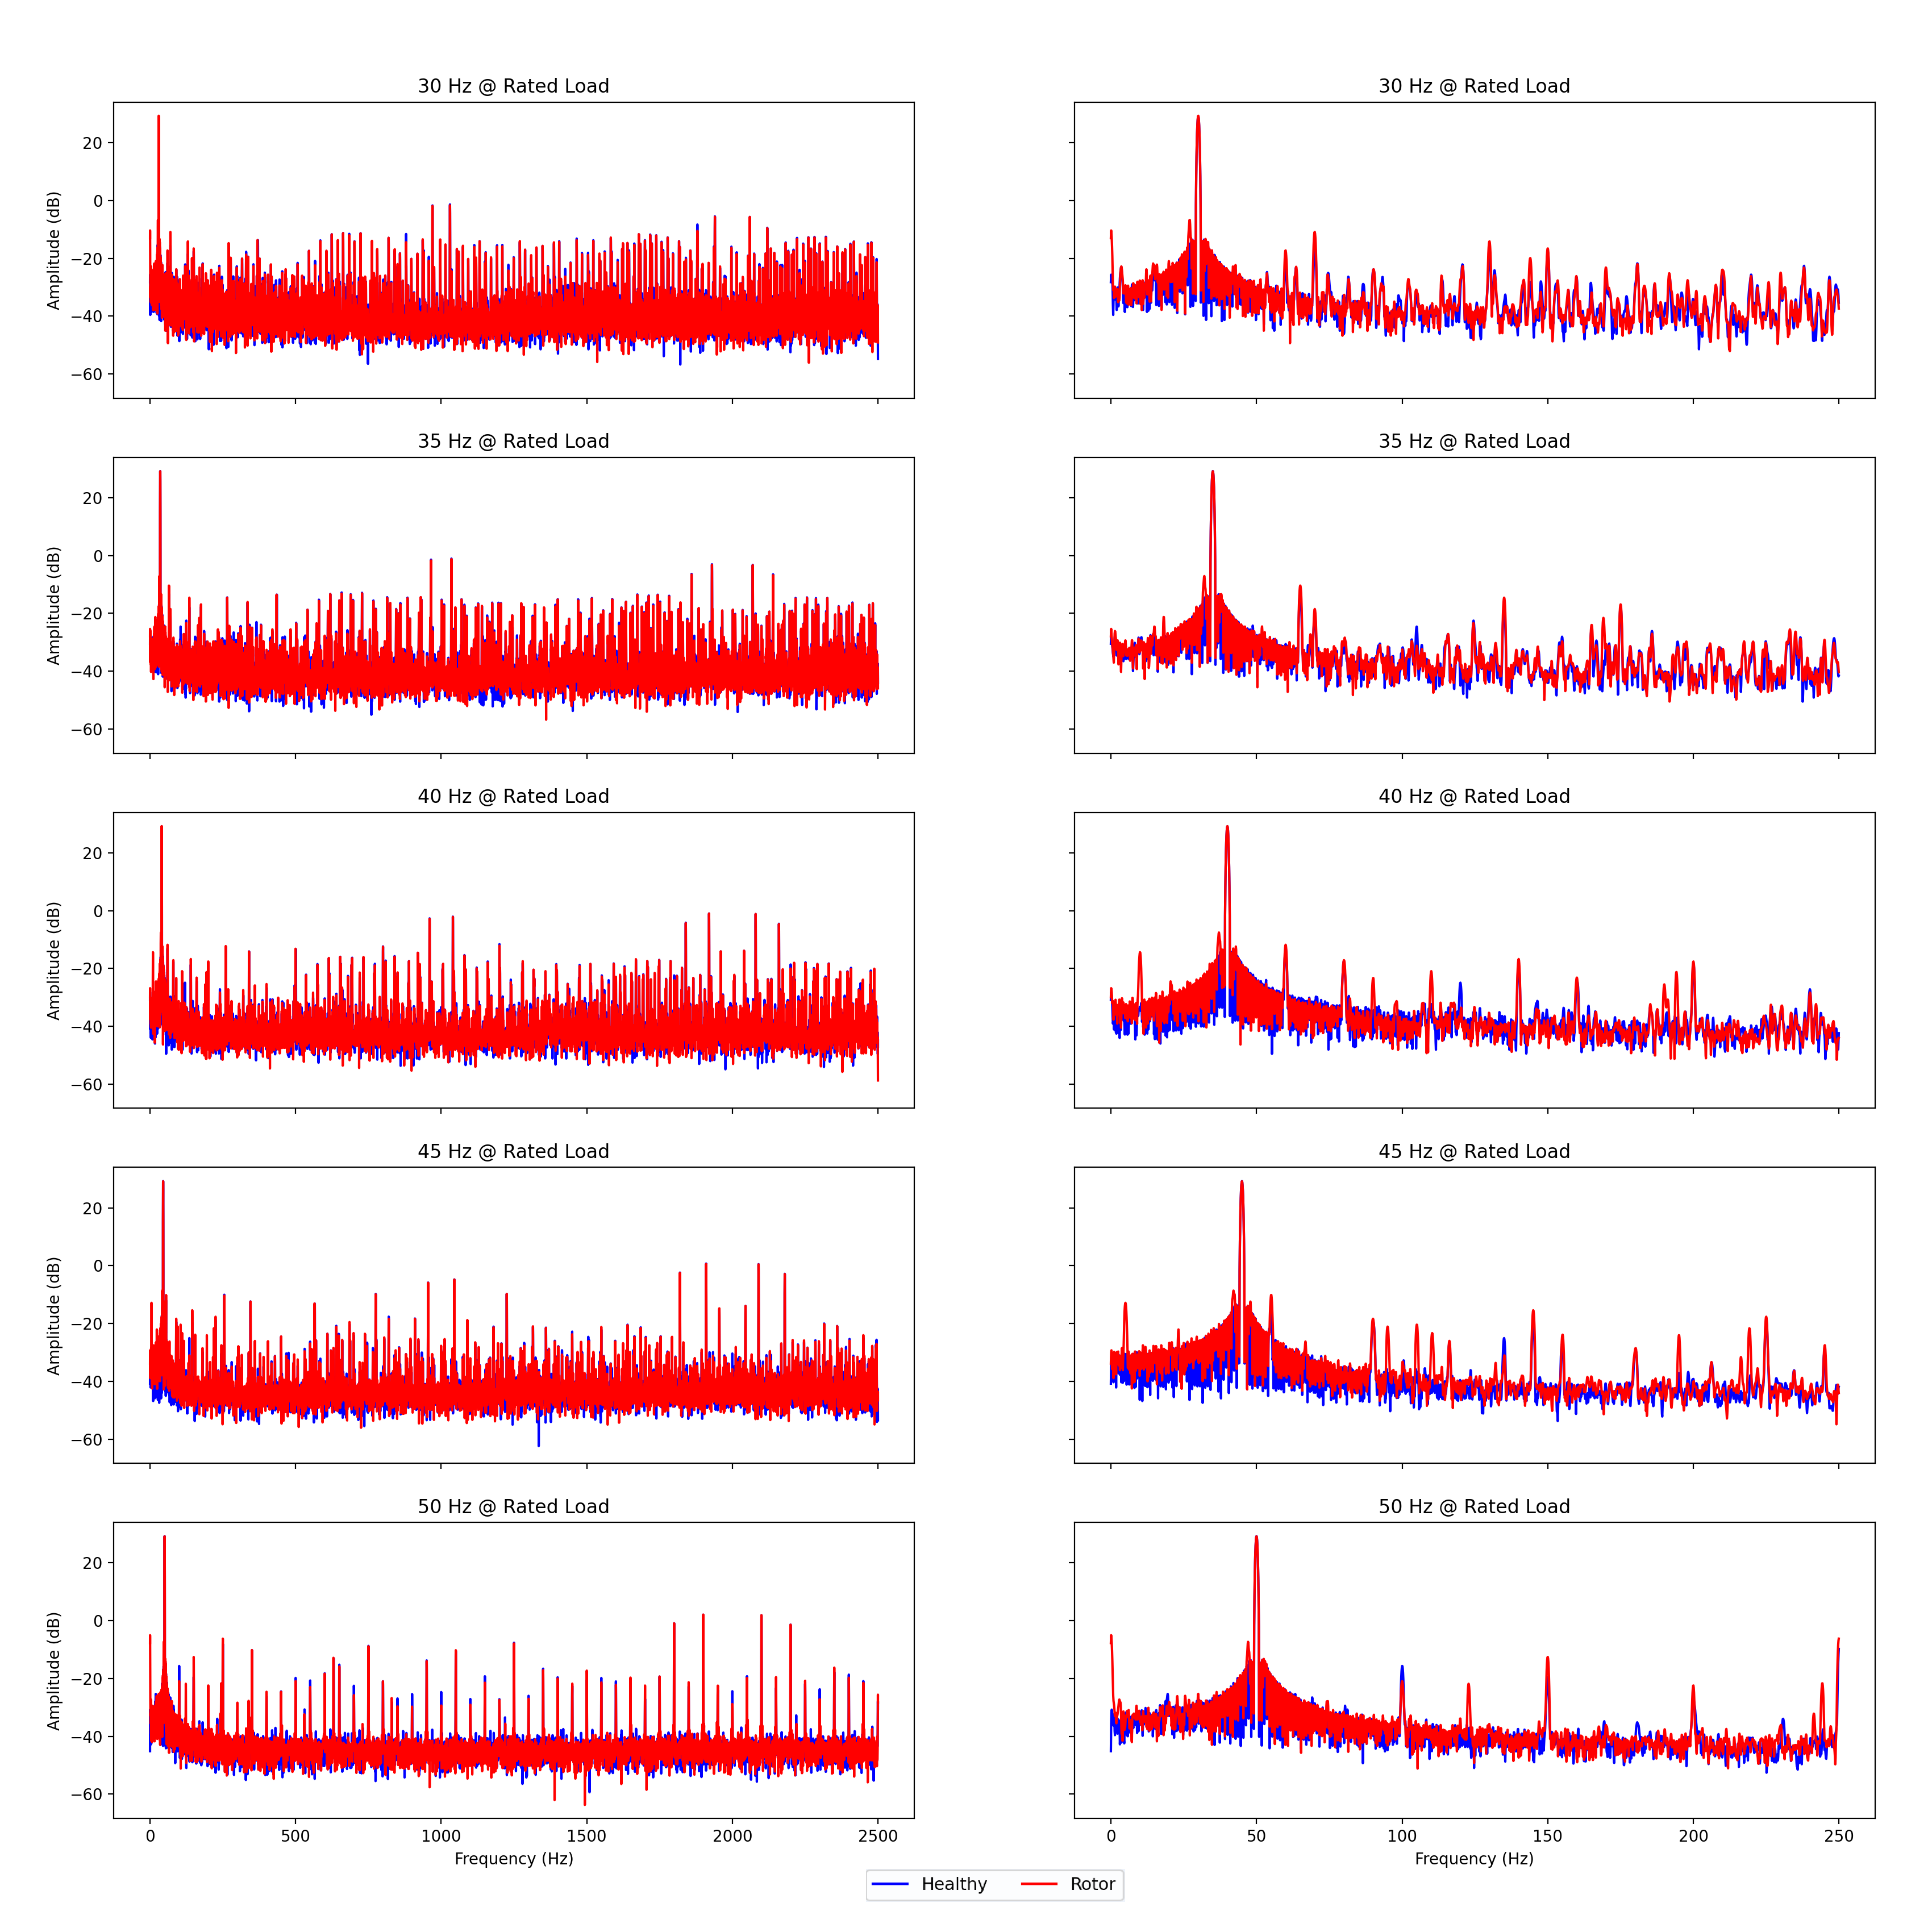
\includegraphics[width=0.75\paperwidth,keepaspectratio=true]{./fig/psdrotor_100.png}
	% sekil3.eps: 0x0 pixel, 300dpi, 0.00x0.00 cm, bb=14 14 1155 740
	\caption{Welch's PSD estimations of healthy and broken rotor bar-fault motor at 75$\%$ of the rated load.}	
	\label{psdrotor100}
\end{figure}
\pagebreak
\begin{figure}[p]
	\centering
	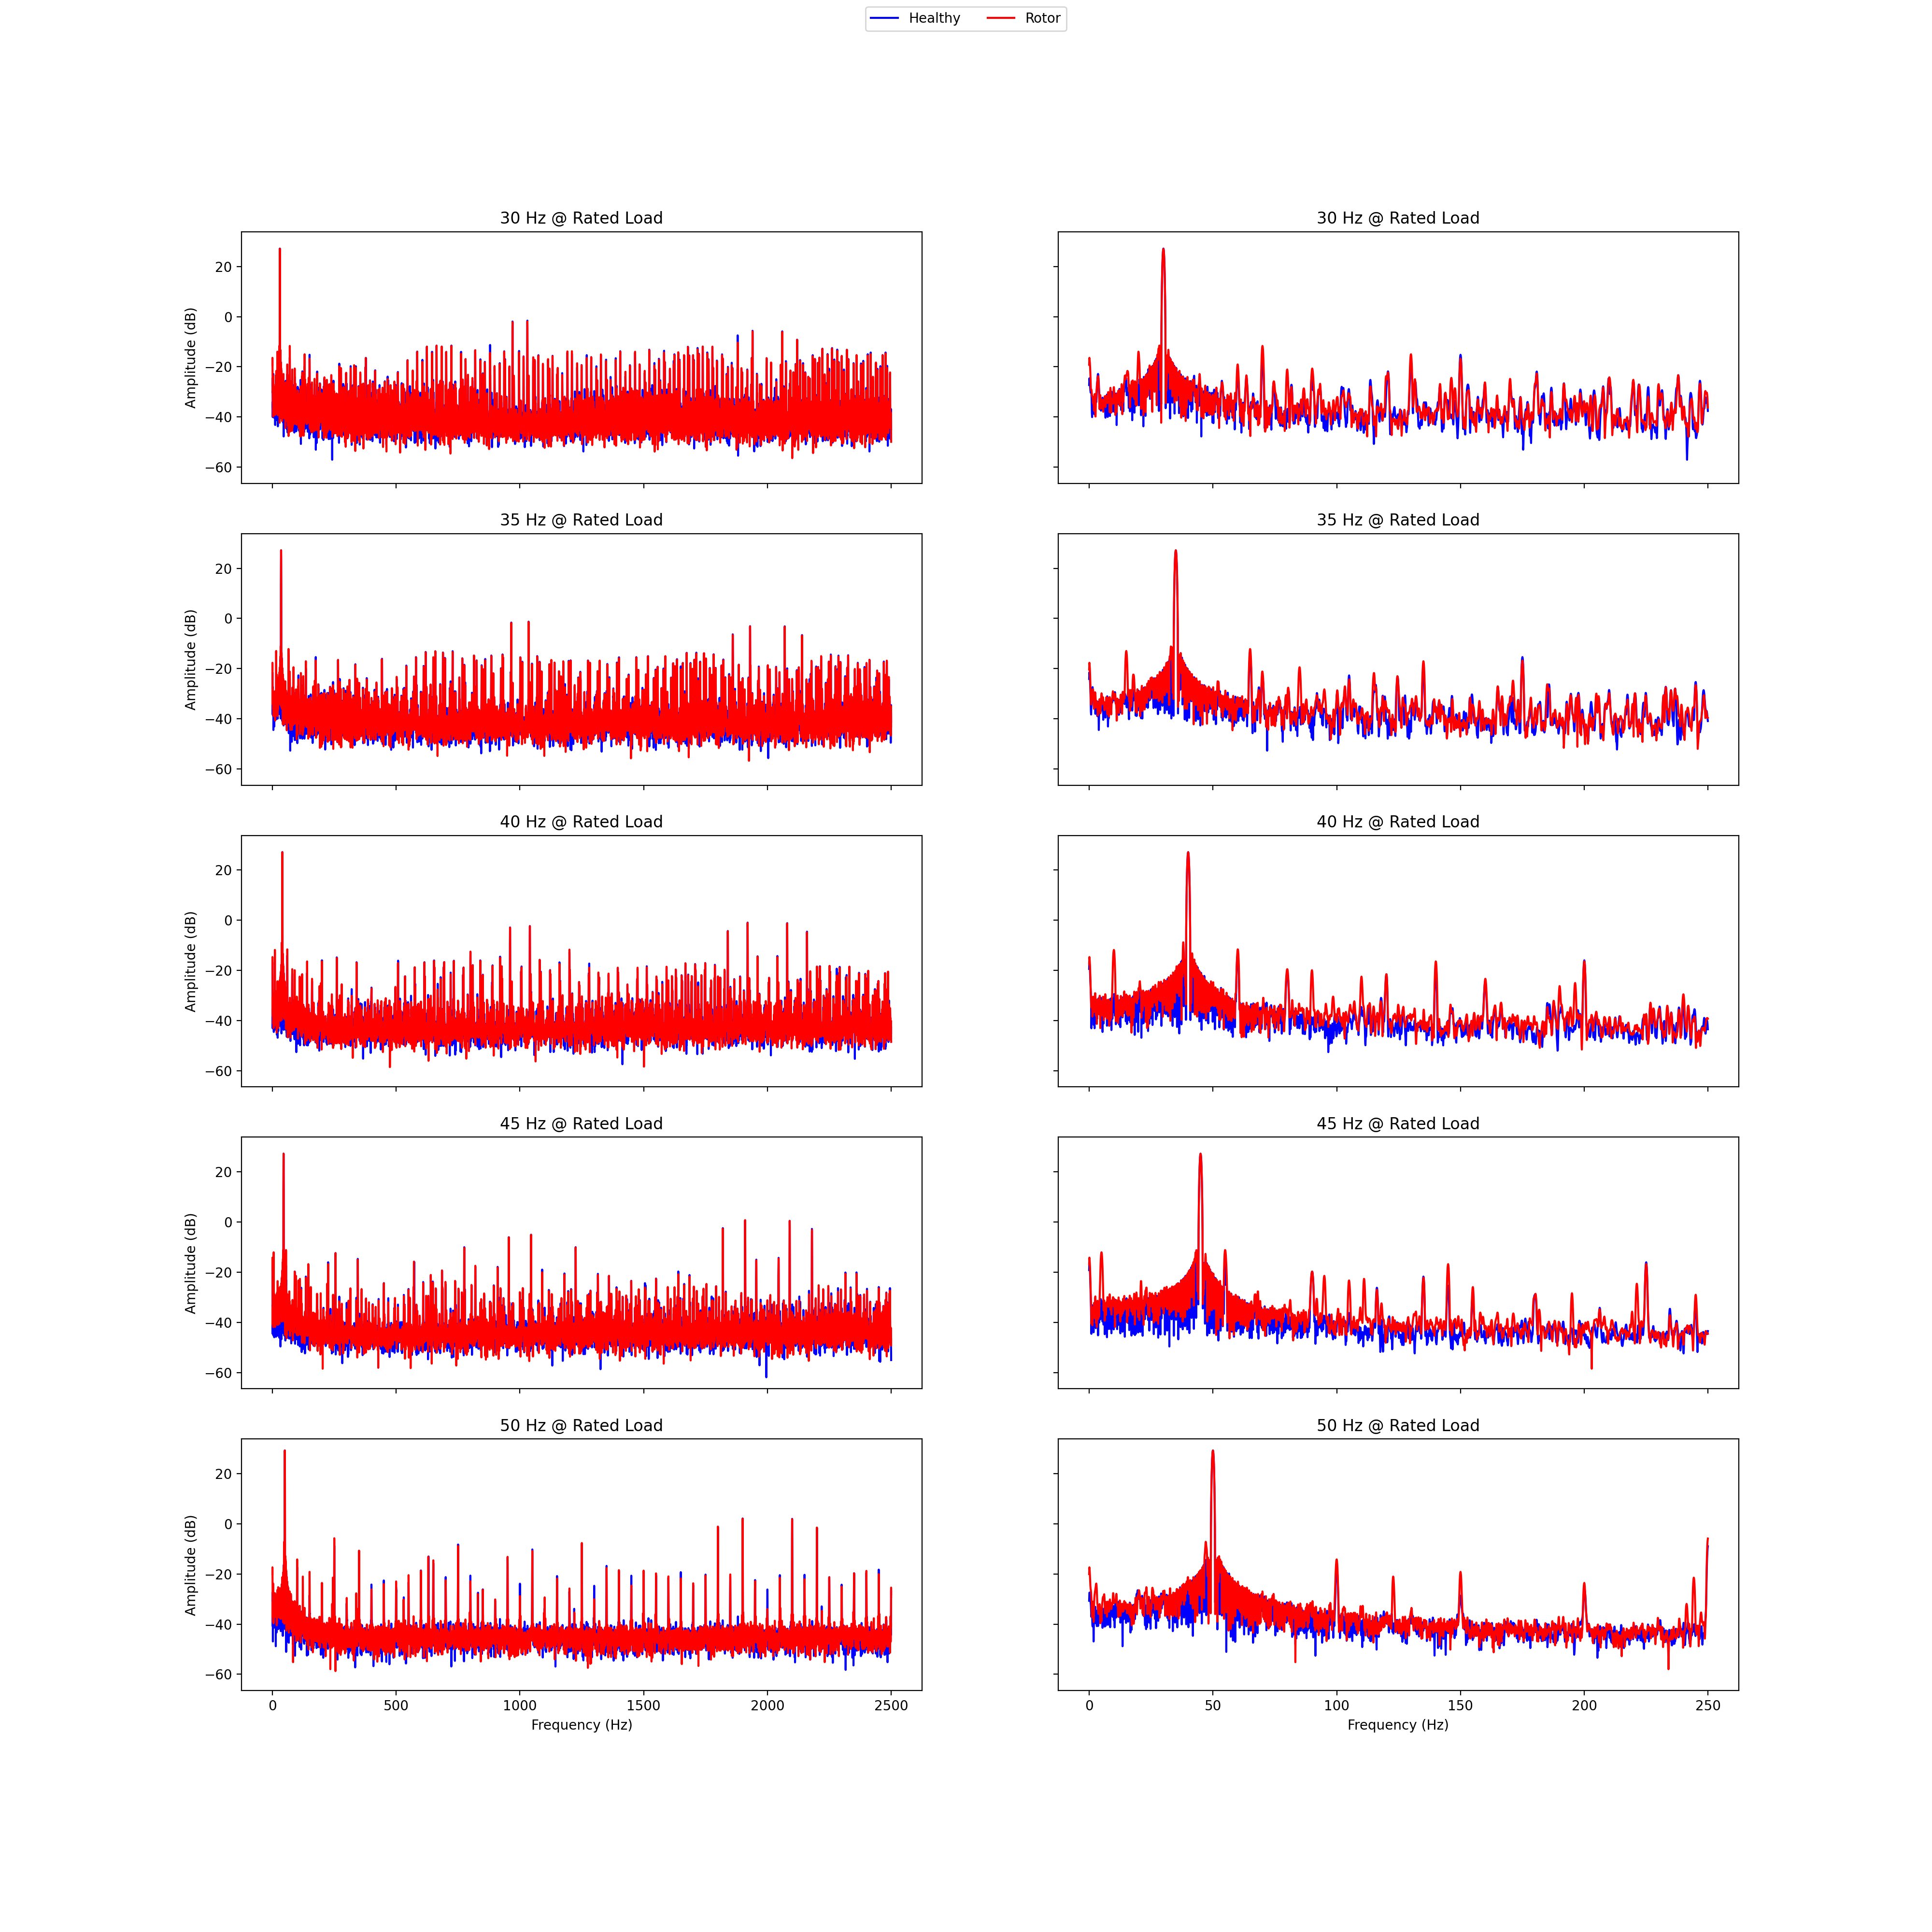
\includegraphics[width=0.75\paperwidth,keepaspectratio=true]{./fig/psdrotor_75.png}
	% sekil3.eps: 0x0 pixel, 300dpi, 0.00x0.00 cm, bb=14 14 1155 740
	\caption{Welch's PSD estimations of healthy and broken rotor bar-fault motor at 75$\%$ of the rated load.}
	\label{psdrotor75}
\end{figure}

